
%% bare_jrnl.tex
%% V1.4b
%% 2015/08/26
%% by Michael Shell
%% see http://www.michaelshell.org/
%% for current contact information.
%%
%% This is a skeleton file demonstrating the use of IEEEtran.cls
%% (requires IEEEtran.cls version 1.8b or later) with an IEEE
%% journal paper.
%%
%% Support sites:
%% http://www.michaelshell.org/tex/ieeetran/
%% http://www.ctan.org/pkg/ieeetran
%% and
%% http://www.ieee.org/

%%*************************************************************************
%% Legal Notice:
%% This code is offered as-is without any warranty either expressed or
%% implied; without even the implied warranty of MERCHANTABILITY or
%% FITNESS FOR A PARTICULAR PURPOSE! 
%% User assumes all risk.
%% In no event shall the IEEE or any contributor to this code be liable for
%% any damages or losses, including, but not limited to, incidental,
%% consequential, or any other damages, resulting from the use or misuse
%% of any information contained here.
%%
%% All comments are the opinions of their respective authors and are not
%% necessarily endorsed by the IEEE.
%%
%% This work is distributed under the LaTeX Project Public License (LPPL)
%% ( http://www.latex-project.org/ ) version 1.3, and may be freely used,
%% distributed and modified. A copy of the LPPL, version 1.3, is included
%% in the base LaTeX documentation of all distributions of LaTeX released
%% 2003/12/01 or later.
%% Retain all contribution notices and credits.
%% ** Modified files should be clearly indicated as such, including  **
%% ** renaming them and changing author support contact information. **
%%*************************************************************************


% *** Authors should verify (and, if needed, correct) their LaTeX system  ***
% *** with the testflow diagnostic prior to trusting their LaTeX platform ***
% *** with production work. The IEEE's font choices and paper sizes can   ***
% *** trigger bugs that do not appear when using other class files.       ***                          ***
% The testflow support page is at:
% http://www.michaelshell.org/tex/testflow/



\documentclass[journal]{IEEEtran}
%
% If IEEEtran.cls has not been installed into the LaTeX system files,
% manually specify the path to it like:
% \documentclass[journal]{../sty/IEEEtran}


% Some very useful LaTeX packages include:
% (uncomment the ones you want to load)


% *** MISC UTILITY PACKAGES ***
%
%\usepackage{ifpdf}
% Heiko Oberdiek's ifpdf.sty is very useful if you need conditional
% compilation based on whether the output is pdf or dvi.
% usage:
% \ifpdf
%   % pdf code
% \else
%   % dvi code
% \fi
% The latest version of ifpdf.sty can be obtained from:
% http://www.ctan.org/pkg/ifpdf
% Also, note that IEEEtran.cls V1.7 and later provides a builtin
% \ifCLASSINFOpdf conditional that works the same way.
% When switching from latex to pdflatex and vice-versa, the compiler may
% have to be run twice to clear warning/error messages.


% *** CITATION PACKAGES ***
%
%\usepackage{cite}
% cite.sty was written by Donald Arseneau
% V1.6 and later of IEEEtran pre-defines the format of the cite.sty package
% \cite{} output to follow that of the IEEE. Loading the cite package will
% result in citation numbers being automatically sorted and properly
% "compressed/ranged". e.g., [1], [9], [2], [7], [5], [6] without using
% cite.sty will become [1], [2], [5]--[7], [9] using cite.sty. cite.sty's
% \cite will automatically add leading space, if needed. Use cite.sty's
% noadjust option (cite.sty V3.8 and later) if you want to turn this off
% such as if a citation ever needs to be enclosed in parenthesis.
% cite.sty is already installed on most LaTeX systems. Be sure and use
% version 5.0 (2009-03-20) and later if using hyperref.sty.
% The latest version can be obtained at:
% http://www.ctan.org/pkg/cite
% The documentation is contained in the cite.sty file itself.


% *** GRAPHICS RELATED PACKAGES ***
%
\ifCLASSINFOpdf
  % \usepackage[pdftex]{graphicx}
  % declare the path(s) where your graphic files are
  % \graphicspath{{../pdf/}{../jpeg/}}
  % and their extensions so you won't have to specify these with
  % every instance of \includegraphics
  % \DeclareGraphicsExtensions{.pdf,.jpeg,.png}
\else
  % or other class option (dvipsone, dvipdf, if not using dvips). graphicx
  % will default to the driver specified in the system graphics.cfg if no
  % driver is specified.
  % \usepackage[dvips]{graphicx}
  % declare the path(s) where your graphic files are
  % \graphicspath{{../eps/}}
  % and their extensions so you won't have to specify these with
  % every instance of \includegraphics
  % \DeclareGraphicsExtensions{.eps}
\fi
% graphicx was written by David Carlisle and Sebastian Rahtz. It is
% required if you want graphics, photos, etc. graphicx.sty is already
% installed on most LaTeX systems. The latest version and documentation
% can be obtained at: 
% http://www.ctan.org/pkg/graphicx
% Another good source of documentation is "Using Imported Graphics in
% LaTeX2e" by Keith Reckdahl which can be found at:
% http://www.ctan.org/pkg/epslatex
%
% latex, and pdflatex in dvi mode, support graphics in encapsulated
% postscript (.eps) format. pdflatex in pdf mode supports graphics
% in .pdf, .jpeg, .png and .mps (metapost) formats. Users should ensure
% that all non-photo figures use a vector format (.eps, .pdf, .mps) and
% not a bitmapped formats (.jpeg, .png). The IEEE frowns on bitmapped formats
% which can result in "jaggedy"/blurry rendering of lines and letters as
% well as large increases in file sizes.
%
% You can find documentation about the pdfTeX application at:
% http://www.tug.org/applications/pdftex


% *** MATH PACKAGES ***
%
%\usepackage{amsmath}
% A popular package from the American Mathematical Society that provides
% many useful and powerful commands for dealing with mathematics.
%
% Note that the amsmath package sets \interdisplaylinepenalty to 10000
% thus preventing page breaks from occurring within multiline equations. Use:
%\interdisplaylinepenalty=2500
% after loading amsmath to restore such page breaks as IEEEtran.cls normally
% does. amsmath.sty is already installed on most LaTeX systems. The latest
% version and documentation can be obtained at:
% http://www.ctan.org/pkg/amsmath


% *** SPECIALIZED LIST PACKAGES ***
%
%\usepackage{algorithmic}
% algorithmic.sty was written by Peter Williams and Rogerio Brito.
% This package provides an algorithmic environment fo describing algorithms.
% You can use the algorithmic environment in-text or within a figure
% environment to provide for a floating algorithm. Do NOT use the algorithm
% floating environment provided by algorithm.sty (by the same authors) or
% algorithm2e.sty (by Christophe Fiorio) as the IEEE does not use dedicated
% algorithm float types and packages that provide these will not provide
% correct IEEE style captions. The latest version and documentation of
% algorithmic.sty can be obtained at:
% http://www.ctan.org/pkg/algorithms
% Also of interest may be the (relatively newer and more customizable)
% algorithmicx.sty package by Szasz Janos:
% http://www.ctan.org/pkg/algorithmicx


% *** ALIGNMENT PACKAGES ***
%
%\usepackage{array}
% Frank Mittelbach's and David Carlisle's array.sty patches and improves
% the standard LaTeX2e array and tabular environments to provide better
% appearance and additional user controls. As the default LaTeX2e table
% generation code is lacking to the point of almost being broken with
% respect to the quality of the end results, all users are strongly
% advised to use an enhanced (at the very least that provided by array.sty)
% set of table tools. array.sty is already installed on most systems. The
% latest version and documentation can be obtained at:
% http://www.ctan.org/pkg/array


% IEEEtran contains the IEEEeqnarray family of commands that can be used to
% generate multiline equations as well as matrices, tables, etc., of high
% quality.


% *** SUBFIGURE PACKAGES ***
%\ifCLASSOPTIONcompsoc
%  \usepackage[caption=false,font=normalsize,labelfont=sf,textfont=sf]{subfig}
%\else
%  \usepackage[caption=false,font=footnotesize]{subfig}
%\fi
% subfig.sty, written by Steven Douglas Cochran, is the modern replacement
% for subfigure.sty, the latter of which is no longer maintained and is
% incompatible with some LaTeX packages including fixltx2e. However,
% subfig.sty requires and automatically loads Axel Sommerfeldt's caption.sty
% which will override IEEEtran.cls' handling of captions and this will result
% in non-IEEE style figure/table captions. To prevent this problem, be sure
% and invoke subfig.sty's "caption=false" package option (available since
% subfig.sty version 1.3, 2005/06/28) as this is will preserve IEEEtran.cls
% handling of captions.
% Note that the Computer Society format requires a larger sans serif font
% than the serif footnote size font used in traditional IEEE formatting
% and thus the need to invoke different subfig.sty package options depending
% on whether compsoc mode has been enabled.
%
% The latest version and documentation of subfig.sty can be obtained at:
% http://www.ctan.org/pkg/subfig


% *** FLOAT PACKAGES ***
%
%\usepackage{fixltx2e}
% fixltx2e, the successor to the earlier fix2col.sty, was written by
% Frank Mittelbach and David Carlisle. This package corrects a few problems
% in the LaTeX2e kernel, the most notable of which is that in current
% LaTeX2e releases, the ordering of single and double column floats is not
% guaranteed to be preserved. Thus, an unpatched LaTeX2e can allow a
% single column figure to be placed prior to an earlier double column
% figure.
% Be aware that LaTeX2e kernels dated 2015 and later have fixltx2e.sty's
% corrections already built into the system in which case a warning will
% be issued if an attempt is made to load fixltx2e.sty as it is no longer
% needed.
% The latest version and documentation can be found at:
% http://www.ctan.org/pkg/fixltx2e


%\usepackage{stfloats}
% stfloats.sty was written by Sigitas Tolusis. This package gives LaTeX2e
% the ability to do double column floats at the bottom of the page as well
% as the top. (e.g., "\begin{figure*}[!b]" is not normally possible in
% LaTeX2e). It also provides a command:
%\fnbelowfloat
% to enable the placement of footnotes below bottom floats (the standard
% LaTeX2e kernel puts them above bottom floats). This is an invasive package
% which rewrites many portions of the LaTeX2e float routines. It may not work
% with other packages that modify the LaTeX2e float routines. The latest
% version and documentation can be obtained at:
% http://www.ctan.org/pkg/stfloats
% Do not use the stfloats baselinefloat ability as the IEEE does not allow
% \baselineskip to stretch. Authors submitting work to the IEEE should note
% that the IEEE rarely uses double column equations and that authors should try
% to avoid such use. Do not be tempted to use the cuted.sty or midfloat.sty
% packages (also by Sigitas Tolusis) as the IEEE does not format its papers in
% such ways.
% Do not attempt to use stfloats with fixltx2e as they are incompatible.
% Instead, use Morten Hogholm'a dblfloatfix which combines the features
% of both fixltx2e and stfloats:
%
% \usepackage{dblfloatfix}
% The latest version can be found at:
% http://www.ctan.org/pkg/dblfloatfix


%\ifCLASSOPTIONcaptionsoff
%  \usepackage[nomarkers]{endfloat}
% \let\MYoriglatexcaption\caption
% \renewcommand{\caption}[2][\relax]{\MYoriglatexcaption[#2]{#2}}
%\fi
% endfloat.sty was written by James Darrell McCauley, Jeff Goldberg and 
% Axel Sommerfeldt. This package may be useful when used in conjunction with 
% IEEEtran.cls'  captionsoff option. Some IEEE journals/societies require that
% submissions have lists of figures/tables at the end of the paper and that
% figures/tables without any captions are placed on a page by themselves at
% the end of the document. If needed, the draftcls IEEEtran class option or
% \CLASSINPUTbaselinestretch interface can be used to increase the line
% spacing as well. Be sure and use the nomarkers option of endfloat to
% prevent endfloat from "marking" where the figures would have been placed
% in the text. The two hack lines of code above are a slight modification of
% that suggested by in the endfloat docs (section 8.4.1) to ensure that
% the full captions always appear in the list of figures/tables - even if
% the user used the short optional argument of \caption[]{}.
% IEEE papers do not typically make use of \caption[]'s optional argument,
% so this should not be an issue. A similar trick can be used to disable
% captions of packages such as subfig.sty that lack options to turn off
% the subcaptions:
% For subfig.sty:
% \let\MYorigsubfloat\subfloat
% \renewcommand{\subfloat}[2][\relax]{\MYorigsubfloat[]{#2}}
% However, the above trick will not work if both optional arguments of
% the \subfloat command are used. Furthermore, there needs to be a
% description of each subfigure *somewhere* and endfloat does not add
% subfigure captions to its list of figures. Thus, the best approach is to
% avoid the use of subfigure captions (many IEEE journals avoid them anyway)
% and instead reference/explain all the subfigures within the main caption.
% The latest version of endfloat.sty and its documentation can obtained at:
% http://www.ctan.org/pkg/endfloat
%
% The IEEEtran \ifCLASSOPTIONcaptionsoff conditional can also be used
% later in the document, say, to conditionally put the References on a 
% page by themselves.


% *** PDF, URL AND HYPERLINK PACKAGES ***
%
%\usepackage{url}
% url.sty was written by Donald Arseneau. It provides better support for
% handling and breaking URLs. url.sty is already installed on most LaTeX
% systems. The latest version and documentation can be obtained at:
% http://www.ctan.org/pkg/url
% Basically, \url{my_url_here}.


% *** Do not adjust lengths that control margins, column widths, etc. ***
% *** Do not use packages that alter fonts (such as pslatex).         ***
% There should be no need to do such things with IEEEtran.cls V1.6 and later.
% (Unless specifically asked to do so by the journal or conference you plan
% to submit to, of course. )

\usepackage{graphics} % for pdf, bitmapped graphics files
\usepackage{epsfig} % for postscript graphics files
\usepackage{mathptmx} % assumes new font selection scheme installed
\usepackage{times} % assumes new font selection scheme installed
\usepackage{amsmath} % assumes amsmath package installed
\usepackage{amssymb}  % assumes amsmath package installed
%\usepackage{amsthm}
\usepackage{bm}
%\usepackage{caption}
\usepackage{mathrsfs}
\usepackage{xcolor}
\usepackage{cite}
\usepackage{threeparttable}
\usepackage{multirow}
\usepackage{bigdelim}
\usepackage{algorithm}
\usepackage{algorithmicx}
\usepackage{algpseudocode}
\usepackage{graphicx}
\usepackage{subfigure}
\usepackage{comment}
\usepackage{array}


% correct bad hyphenation here
\hyphenation{op-tical net-works semi-conduc-tor}


\begin{document}
%
% paper title
% Titles are generally capitalized except for words such as a, an, and, as,
% at, but, by, for, in, nor, of, on, or, the, to and up, which are usually
% not capitalized unless they are the first or last word of the title.
% Linebreaks \\ can be used within to get better formatting as desired.
% Do not put math or special symbols in the title.
\title{Cellular Decomposition for Non-repetitive Coverage Task with Minimum Discontinuities}
%
%
% author names and IEEE memberships
% note positions of commas and nonbreaking spaces ( ~ ) LaTeX will not break
% a structure at a ~ so this keeps an author's name from being broken across
% two lines.
% use \thanks{} to gain access to the first footnote area
% a separate \thanks must be used for each paragraph as LaTeX2e's \thanks
% was not built to handle multiple paragraphs
%

%\author{Michael~Shell,~\IEEEmembership{Member,~IEEE,}
%        John~Doe,~\IEEEmembership{Fellow,~OSA,}
%        and~Jane~Doe,~\IEEEmembership{Life~Fellow,~IEEE}% <-this % stops a space
%\thanks{M. Shell was with the Department
%of Electrical and Computer Engineering, Georgia Institute of Technology, Atlanta,
%GA, 30332 USA e-mail: (see http://www.michaelshell.org/contact.html).}% <-this % stops a space
%\thanks{J. Doe and J. Doe are with Anonymous University.}% <-this % stops a space
%\thanks{Manuscript received April 19, 2005; revised August 26, 2015.}}

\author{Tong Yang$^1$, Jaime Valls Miro$^2$~\IEEEmembership{Member,~IEEE}, Qianen Lai$^1$, Yue Wang$^{1*}$ and Rong Xiong$^1$
\thanks{$^1$ Tong Yang, Qianen Lai, Yue Wang and Rong Xiong are with the State Key 
Laboratory of Industrial Control and Technology, Zhejiang University, P.R. China. 
%Yue Wang is the corresponding author {\tt\small wangyue@iipc.zju.edu.cn}. Rong Xiong is the co-corresponding author {\tt\small rxiong@zju.edu.cn}.
}
\thanks{$^2$ Jaime Valls Miro is with the Centre for Autonomous Systems (CAS), University of Technology Sydney (UTS), Sydney, Australia.}
\thanks{$^*$ Corresponding Author. \newline \indent
E-mail address: {\tt\small wangyue@iipc.zju.edu.cn}}
}

% note the % following the last \IEEEmembership and also \thanks - 
% these prevent an unwanted space from occurring between the last author name
% and the end of the author line. i.e., if you had this:
% 
% \author{....lastname \thanks{...} \thanks{...} }
%                     ^------------^------------^----Do not want these spaces!
%
% a space would be appended to the last name and could cause every name on that
% line to be shifted left slightly. This is one of those "LaTeX things". For
% instance, "\textbf{A} \textbf{B}" will typeset as "A B" not "AB". To get
% "AB" then you have to do: "\textbf{A}\textbf{B}"
% \thanks is no different in this regard, so shield the last } of each \thanks
% that ends a line with a % and do not let a space in before the next \thanks.
% Spaces after \IEEEmembership other than the last one are OK (and needed) as
% you are supposed to have spaces between the names. For what it is worth,
% this is a minor point as most people would not even notice if the said evil
% space somehow managed to creep in.


% The paper headers
\markboth{This paper is concurrently submitted for TMech and AIM 2020 Presentation}{}
%\markboth{Journal of \LaTeX\ Class Files,~Vol.~14, No.~8, August~2015}%
%{Tong \MakeLowercase{\textit{et al.}}: Cellular Decomposition for Non-repetitive Coverage Task Ensuring Least Discontinuities}
% The only time the second header will appear is for the odd numbered pages
% after the title page when using the twoside option.
% 
% *** Note that you probably will NOT want to include the author's ***
% *** name in the headers of peer review papers.                   ***
% You can use \ifCLASSOPTIONpeerreview for conditional compilation here if
% you desire.


% If you want to put a publisher's ID mark on the page you can do it like
% this:
%\IEEEpubid{0000--0000/00\$00.00~\copyright~2015 IEEE}
% Remember, if you use this you must call \IEEEpubidadjcol in the second
% column for its text to clear the IEEEpubid mark.

% use for special paper notices
%\IEEEspecialpapernotice{(Invited Paper)}


% make the title area
\maketitle

% As a general rule, do not put math, special symbols or citations
% in the abstract or keywords.
\begin{abstract}
A mechanism to derive non-repetitive coverage path solutions with a proven minimal number of discontinuities is proposed in this work, with the aim to avoid unnecessary, costly end effector lift-offs for manipulators. The problem is motivated by the automatic polishing of an object. Due to the non-bijective mapping between the workspace and the joint-space, a continuous coverage path in the workspace may easily be truncated in the joint-space, incuring undesirable end effector lift-offs. Inversely, there may be multiple configuration choices to cover the same point of a coverage path through the solution of the Inverse Kinematics. 
The solution departs from the conventional local optimisation of the coverage path shape in task space, or choosing appropiate but possibly disconnected configurations, to instead explicitly explore the least number of discontinuous motions through the analysis of the structure of valid configurations in joint-space. The two novel contributions of this paper include proof 
that the least number of path discontinuities is predicated on the surrounding environment, independent from the choice of the actual coverage path; thus has a minimum. And an efficient finite cellular decomposition method to optimally divide the workspace into the minimum number of cells, each traversable without discontinuities by any arbitrary coverage path within. 
%The algorithm is operational in any dimension, and we illustrate it through polishing tasks.
Extensive simulation examples and real-world results on a 5 DoF manipulator are presented to prove the validity of the proposed
strategy in realistic settings.
\end{abstract}

% Note that keywords are not normally used for peerreview papers.
\begin{IEEEkeywords}
Cellular Decomposition, Non-repetitive Coverage Task, Non-redundant Manipulator
\end{IEEEkeywords}


% For peer review papers, you can put extra information on the cover
% page as needed:
% \ifCLASSOPTIONpeerreview
% \begin{center} \bfseries EDICS Category: 3-BBND \end{center}
% \fi
%
% For peerreview papers, this IEEEtran command inserts a page break and
% creates the second title. It will be ignored for other modes.
\IEEEpeerreviewmaketitle

\section{Introduction}
% The very first letter is a 2 line initial drop letter followed
% by the rest of the first word in caps.
% 
% form to use if the first word consists of a single letter:
% \IEEEPARstart{A}{demo} file is ....
% 
% form to use if you need the single drop letter followed by
% normal text (unknown if ever used by the IEEE):
% \IEEEPARstart{A}{}demo file is ....
% 
% Some journals put the first two words in caps:
% \IEEEPARstart{T}{his demo} file is ....
% 
% Here we have the typical use of a "T" for an initial drop letter
% and "HIS" in caps to complete the first word.

\IEEEPARstart{T}{he} non-repetitive \textit{coverage task} of a given object is an important application carried out by manipulators.
This is for instance the case of inspecting a surface for defects at close 
range~\cite{molina2017defects}, painting~\cite{li2011painting}, deburring~\cite{xie2016grinding} or polishing~\cite{tian2016polishing}. 
The task is effectively encapsulated as the generic coverage path planning (CPP)~\cite{choset2001coverage}~\cite{galceran2013a} problem, which requires for the end-effector (EE) to traverse over all the points that define the surface of a given object exactly one time, whilst usually fulfilling additional task-specific constraints (e.g. sustaining a desired orientation of the EE with respect to the surface, maintain contact or exerting a constant EE force/torque). 
This is in contrast to error reduction-driven  motion planning schemes for robotic tasks requiring high precision, such as repetitive motion planning (RMP)~\cite{xie2019rmp}, or so-called cycling motion generation (CMG) schemes~\cite{xie2020cyclic}, notably attractive for repetitive automated industrial production processes.

Typically, joint-space dimension is higher than the workspace's, % such as using a non-redundant manipulator to polish a surface, 
and the Inverse Kinematic (IK) mapping between task and joint space is thus non-bijective.  
%(unique one-to-one correspondences between input-output domains can not be established). 
%Fixed <jvm> I believe this is always the case and we can say so this way  - Tong pls share your view responding to this comment 
% <ty> Yes, the problem of multiple solutions always exists for the revolute joint, and the usage of "non-bijective" is always valid. 
% Yue Wang thought "bijective" is not appropriate, since the mapping is not valid on the whole task-space and the joint-space, but we didn't find a word to express it. Now that you restrict "input-output domains", then both "bijective" and "non-bijective" make sense. 
As a result, planning in the higher dimension joint-space cannot ensure non-repetitive visiting, 
%\begin{color}{blue}
%with the task-to-joint mapping being non-injective, 
%\end{color}
and coverage paths are thus more suited to be designed directly in the workspace domain~\cite{Oriolo2005Motion}.  
% <ty> (1) Are the above two sentences repeated? so we can omit "with the task-to-joint mapping being non-injective"
%      (2) if the sentence is necessary for detailed explanation, then "task-to-joint" should be "joint-to-task". 
\begin{figure}[t]
\centering
\subfigure[Relationship between joint- and work-space.]{
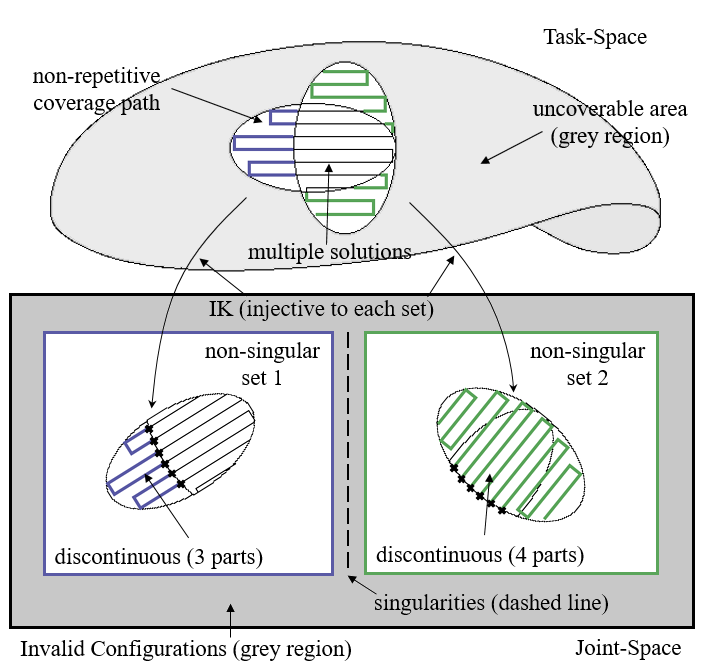
\includegraphics[width = 0.4\textwidth]{figures/other_figures/fig1_mark_singular}
}
\subfigure[Greedy solution example]{
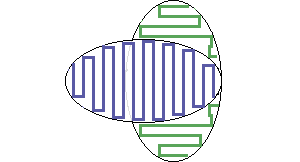
\includegraphics[width = 0.2\textwidth]{figures/other_figures/greedy}
\label{fig:greedy}
}
\subfigure[Optimal solution example]{
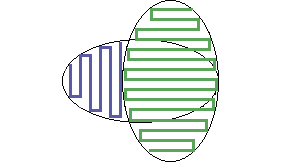
\includegraphics[width = 0.2\textwidth]{figures/other_figures/optimal}
\label{fig:optimal}
}
\caption{(a) Illustration of the coverage task problem and the relationship between joint- and work-space. 
Different colours denote disjoint sets of non-singular 
%multi-dimensional 
joint configurations (arbitrarily, blue may for instance represent those with 
elbow-up, whilst green may represent elbow-down), and their corresponding path in the workspace. 
The coloured segments of the arbitrary coverage path shown in black have unique IK solutions. However, multiple IK solutions exist for the intersecting area shown in black.
%thus requiring further planning decisions. 
The underlying continuous coverage path sought out thus becomes intermittent in the workspace after mapping onto the joint-space.
In this example, whatever choice among the multiple IK solutions, six discontinuities are required 
(depicted by black crosses), since the path has three separate segments in set $1$, and four in set $2$. 
The case where the joint-space solutions are taken in full from set 2 (green) is depicted.
(b) Starting from a configuration belonging to set $1$, without explicitly calculating the reachable boundary of each set, the boundary of the set $2$ within the reachable area of set $1$ is unknown. So a greedy strategy will fully cover the set $1$, dividing the uncovered region into two parts, leading to an extra lift-off. 
On the other hand, although at first sight it may appear the same as using the greedy strategy starting from set $2$. (c) illustrates the concept of CPP optimality in the joint space, whereby the continuity of the reachable area is explicitly considered, thus producing a coverage path with a single EE lift-off.} 
\label{fig1}
\vspace{-0.5cm}
\end{figure}

Yet what constitutes a continuous coverage path in the workspace may easily end up truncated into many seemingly \textit{intermittent} sections after mapping them back onto the joint-space, with undersirable path discontinuities, as graphically illustrated by Fig.~\ref{fig1}. This is also the case if a simplistic greedy strategy is followed, as the example depicted in Fig.~\ref{fig:greedy}, whereby a complete path in task space that solves for all possible configurations leads to unnecessary lift-offs to accomplish full coverage. 

Singularities have been proven to be at the origin of these bifurcations of the joint-space~\cite{porta2010path}~\cite{Porta2012Randomized}, sitting at the intersection of different configurations (e.g. elbow-up and elbow-down).
Notwithstanding singularities, for non-redundant manipulators, non-singular configurations thus form disjoint sets in the joint-space, as illustrated in Fig.~\ref{fig1}, and continuous joint-space paths between sets must then visit singularities along the way for full coverage. The problem is further compounded by additional task constraints, most notably obstacles, which produce usable configurations further divided into many disjoint sets, inevitably incurring undesirable ``jumps'' between sets for successful coverage, as very rarely the whole workspace ends up mapped into a single set.  
%, inevitably incurring undersirable lift-offs. 

This work advocates for the minimisation of the cost incurred on these path discontinuities, which can significantly 
outweigh any improvements proposed in the literature that may occur locally in the task space when it comes 
to coverage~\cite{hassan2018a}. This is perhaps more apparent for the case of the uniform polishing task motivating this work, 
as that means lifting the EE off the object's surface, adjusting the pose of the manipulator to the new configuration, and landing back into contact with the surface again.
This may be not only sub-optimal for the speedy completion of the CPP task, but also introduces potentially avoidable complexity in transitioning between position and force/torque control~\cite{mirrazavi2018a}~\cite{solanes2018adaptive}~\cite{solanes2019robust} % <jvm> add all, reduce if space needed at the end ... I need it!! removed: ~\cite{cheah2003brief}~\cite{heck2015switched}
during the coverage task. 


In this work, a mechanism is proposed to address this shortcoming and derive CPP solutions with a proven minimal number of discontinuities, with the aim to avoid unnecessary, costly EE lift-offs. 
The solution departs from locally optimising the shape of the coverage path in task space, or choosing appropriate but possibly disconnected configurations, but explicitly seeking for least number of discontinuous motions through a novel cellular decomposition analysis of the structure of valid configurations in the joint-space. A conceptual illustration is given in Fig.~\ref{fig:alg_role}.
%
\begin{comment}
The work is predicated on the fact that singularities have been proven to be the cause of bifurcation of the joint-space~\cite{porta2010path}~\cite{Porta2012Randomized}, i.e. sitting at the intersection of different configurations (e.g. elbow-up and elbow-down).
Notwithstanding singularities, for non-redundant manipulators, non-singular configurations thus form disjoint sets in the joint-space, as was illustrated by the earlier example in Fig.~\ref{fig:alg_role}. 
Moreover, due to task constraints (obstacles, joint limits, etc), commonly the whole workspace cannot be mapped into a single set, which then implies that continuous joint-space paths between sets must visit some singularities along the way, inevitably incurring undersirable lift-offs. 
However, manipulators are locally omni-directional in the joint-space, and configurations corresponding to a segment of coverage path without lift-off have high dimensional continuity in the joint-space, independently of their sequencing order. 
Hence, instead of considering the design of a coverage path in the traditional sense, this work considers the global optimal cellular decomposition problem in joint-space to incur joint-space partitions with minimum sets. 
It is further noted that IK mapping from the reachable points in the workspace to a single set of configurations is injective, since there is no non-singular path connecting two configurations whose EEs are at a same point. 
As such, colouring a point in the surface to be covered means selecting a given IK solution for it, and the planning problem is transfered to designing a colour scheme for a topological configuration graph.
In that way, the key concern is the joint-space continuity of the cells, and by efficiently discarding equivalent cellular decompositions, this work proves that total number of different cellular decompositions is finite, thus all optimal solutions are finitely solvable. 
\end{comment}
%
\begin{comment}
% <ty> I guess you want to write like this (in the tealed paragraph)
\begin{color}{blue}
From the observation in Fig.~\ref{fig1}, the problem cannot be relieved through (local) adjustment of the coverage path in the task-space, thus it must be solved in the joint-space. 
Besides, we notice that the configurations corresponding to a piece of coverage path without lift-off have high dimensional continuity in the joint-space~\cite{porta2010path}~\cite{Porta2012Randomized}, 
which is independent to their order. Hence, instead of considering the design of the coverage path, we can instead only consider the optimal cellular decomposition problem in the joint-space. 
Note that here the discussion is restricted in low dimension (because the manipulator is non-redundant), the algorithm for ``all valid configurations'' is computational acceptable. % <jvm> NOTE: this comment about computational tractability to be briefly added, perhaps to discussion?? here in the middle breaks the flow and is not helpful to understand the problem
We further notice that the IK mapping from the reachable points in the task-space to a single set of configuration is injective. 
This motivates us to formulate the problem of joint-space path planning back into the task-space. 
Finally, since our concern is only the joint-space continuity of the cells, through discarding some equivalent cellular decompositions, we prove that the number of different cellular decompositions is finite, thus all optimal solutions are finitely solvable. 
\end{color}
\end{comment}
%
The two novel contributions of this paper can be summarised as: 
\begin{enumerate}
\item Proving that the minimum number of path discontinuities, or ``lift-offs'', for the non-repetitive coverage task with non-redundant manipulators is independent of the actual choice of coverage path. 
Instead, it is predicated on the surrounding environment - the relative pose between manipulator, object and the presence of any obstacles - and this motivates to formulate the problem as a global cellular decomposition process.
On a side note, this also implies that the proposed scheme can be exploited as a criterion to evaluate the most advantageous placement of a manipulator, or object to be manipulated (e.g. polished, painted), both in a fixed configuration (automated production line), or in a mobile manipulation environment. 
\item Proposing an effective finite cellular decomposition method to divide a worskpace surface into the least number of cells whereby each is ensured to be traversable by any arbitrary inner path without incurring discontinuities.
\end{enumerate}


\begin{figure}[t]
\centering
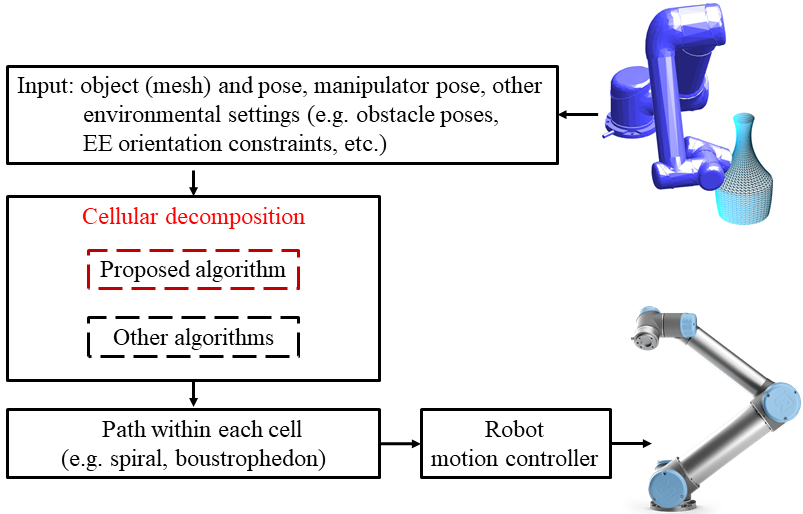
\includegraphics[width = 0.9\columnwidth]{figures/other_figures/relation_3}
\caption{The role of the novel algorithm for the coverage task. The proposed instrument is compatible with any other existing cellular decomposition solutions whilst also 
elliciting a minium number of path discontinuities due to pose reconfigurability.} 
%Embedded with a conventional physical coverage path generator (e.g., the sprial path and the boustrophedon path) in each cell, the algorithm is end-to-end. }
\label{fig:alg_role}
\end{figure}

The remainder of this paper\footnote{A video \label{video} illustrating the concepts and results hereby described can be found here: https://www.youtube.com/watch?v=gyvXin60cCQ\&feature=youtu.be} 
is organised as follows. Section~\ref{sectionrelatedwork} reviews existing literature. 
Section~\ref{sectionproblemformulation} describes the proposed abstraction of the problem into a topological graph of surface cells corresponding 
to feasible, continuous configurations, hence administering the tools to prove that the number of path discontinuities for the CPP problem can be made independently to the eventual coverage path chosen. % <ty> require update, leave it to the last? 
Section~\ref{sectionenumerativesolver} goes into further details about the process of finitely resolving the surface into cell elements, whilst 
Section~\ref{sectioniterativesolver} reports on the proposed iterative strategy to build on the cell elements to ensure CPP with a minimum number of discontinuitues. Experimental results from simulations and on an actual non-reduntant manipulator are collected in Section~\ref{sectionexperiment}, with final concluding remarks gathered in Section~\ref{sectionconclusion}. 


\section{Related Work}\label{sectionrelatedwork}
Almost all state-of-the-art methods to solve the CPP problem first divide the robot's workspace area and then solve the CPP problem in each cell, so called cellular decomposition, which is generally further divided into two categories: exact cellular decomposition methods~\cite{lumelsky1990dynamic} and Morse-based cellular decomposition methods~\cite{choset2000exact}~\cite{Acar2002Morse}. 
Exact cellular decomposition methods divide the free space into several simple, easy sub-regions, and use conventional coverage paths, such as trapezoidal~\cite{choset2005principles} or the boustrophedon paths~\cite{choset1998coverage}~\cite{choset2000coverage}, to finish coverage in each cell. 
Morse-based cellular decomposition methods apply divisions of the free space based on the critical points of Morse functions to present more flexible shapes for cells over those extracted by exact cellular decomposition. 
%Fixed <jvm> Tong  I miss a reference to generalised voronoi diagrams here - I had a go, pls review and cite. And maybe also Delaunay triangulation coverage if you can find a good ref, but within this context of cellular decomposition for full coverage, otherwise leave out
A combination of Morse decomposition and Voronoi diagrams~\cite{choset2000sensor-based} has also been proposed, particularly fitting to 
cover vast open spaces and narrow areas simultaneously.

Optimality of CPP algorithms mainly focus on metrics such as path length and time to completion.
Atkar \textit{et al.}~\cite{Atkar2003Towards} optimised the coverage path through chossing optimal starting points. 
Huang~\cite{huang2001optimal} reduced movement cost by remaining on straight paths as long as possible thus minimising the number of turns. 
Jimenez \textit{et al.}~\cite{jimenez2007optimal} used a genetic algorithm to achieve optimal coverage. 
Whilst generic, the context of these coverage works has almost invariably been motivated by mobile robots operating on 2- or 2.5-dimensional terrains. However, for manipulator, this essay advocates avoiding unnecessary path lift-off discontinuities as that decidedly outweighs any other performance metric improvement that may be achieved during the coverage process, e.g. by switching between differing geometric paths such as boustrophedon and spirals as proposed in the works of Hassan and Liu~\cite{hassan2018a}. 
These discontinuities in the CPP task are inherent to the kinematics of manipulator mechanisms, and as such the algorithms designed for mobile robots do not need to deal with this problem. 
%\begin{color}{blue}
We notice that~\cite{paus2017a} considered the pose 
optimisation of a mobile manipulator for coverage, searching for a valid criterion for the adequacy of the relative pose between manipulator and object(s) to be handled, under the assumption that repositioning the robot is costly and that simultaneous repositioning and end-effector motion is not desired. 
%\end{color}
% <jvm> Tong, I don't think you attended to my earlier comment about this: what can we say we contribute differently vs this work? it may look the same to the reviewer. If they use a different metric and disregard lift offs, that would be sufficient to say here so our propostion stands firm. 

\section{Problem Formulation}\label{sectionproblemformulation}
In this section, we first state the problem of optimal coverage path planning ensuring least number of discontinuites.
The problem is tailored to a polishing task with the introduction of additional task-specific constraints, as per the motivation of this work. 
These could be waived for a more generic exercise. 
% <jvm> I omit intentionally, but could leave: resulting in wider topological search spaces.
Then, we show that the least number of discontinuities is independent of the choice of physical coverage path, 
so the original problem is transformed to an optimal cellular decomposition problem. 
Finally, the minimisation problem is further transformed to a colouring problem of the derived graph ensuring least number of different colours. 

\begin{figure}[t]
\centering
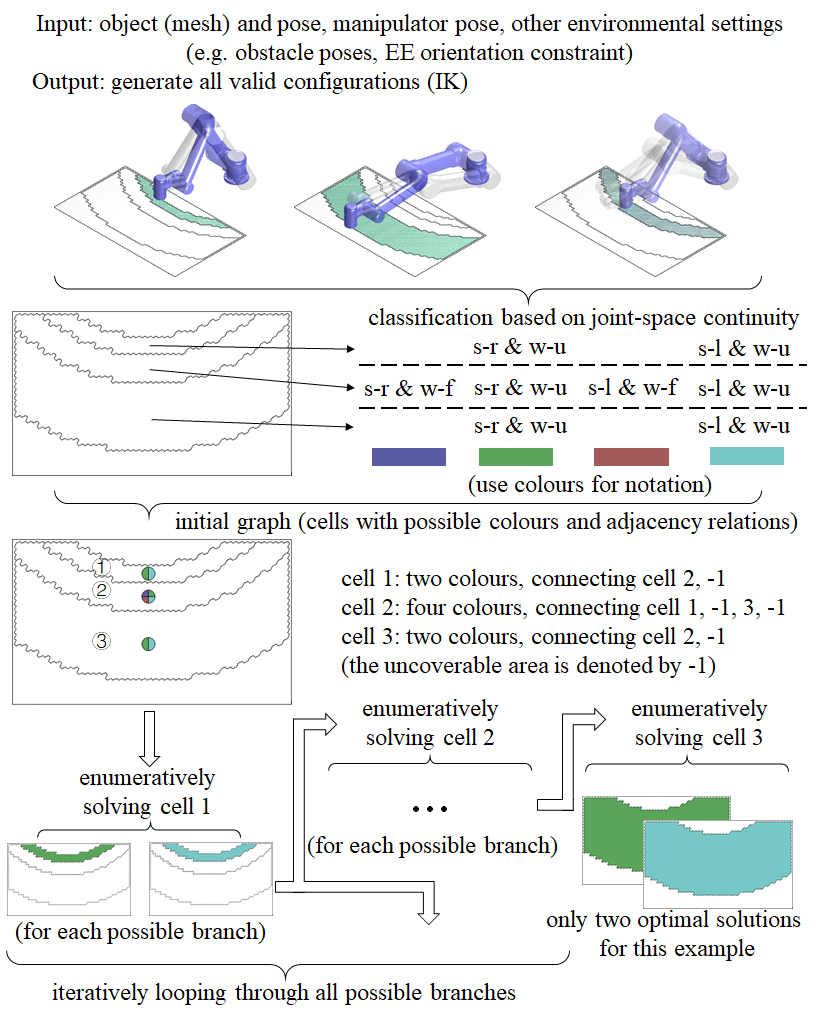
\includegraphics[width = 0.48\textwidth]{figures/other_figures/newflowchart_2}
\caption{Flow chart of the proposed coverage problem solver for optimal lift-off. 
The top section illustrates the different possilbe IK solutions to cover the same surface points. The vivid robot depiction shows the most common class of configuration: shoulder-right - \textit{(s-r)} \& \textit{(w-u)} - wrist-unflipped, able to reach the three cyan areas on the flat surface. Configuration shoulder-left \textit{(s-l)} \& \textit{(w-u)}, shown shaded on the left-most figure) can also reach the same areas. Two additional configurations (shown shaded on the right-most figure), \textit{(s-r)} \& \textit{(w-f)} - wrist-flipped, and \textit{(s-l \& w-f)} are also valid, although they can only cover the middle part of the reachable area, in shaded cyan. An unpainted surface section indicates unreachable by any configuration. Each robot configuration is uniquely denoted, illustrated by a different colour.\protect\\ 
In collecting all valid configurations, since the manipulator is non-redundant, the space of valid configurations has the same 2-dimension as the task-space, and it is thus computable based on IK relations. A corresponding topological graph is generated based on the distribution of possible colours, and a solver is developed to reach all optimal solutions in proven finite steps. More details of the iterative solver process are provided in the text and in Fig.~\ref{fig:solver}.
%it is easy to see that there are only two optimal solutions. 
}
%Flow chart of the proposed modelling of the coverage problem and the methodology for solving. For abbreviation: shoulder-left(s-l), shoulder-right(s-r), wrist-flipped(w-f), wrist-unflipped(w-u). In collecting all valid configurations, since the manipulator is non-redundant, the space of the valid configurations has the same dimension as the task-space (2D) but not the joint-space (5D), thus is computable based on IK relations. For the coverage task using 5 DoF manipulator, the joint-space continuity has intuitive physical meaning (and denoted by different colours): shoulder-left/right and wrist-flipped/unflipped. And a corresponding initial topological graph is generated based on the distribution of possible colours. An iterative solver is proposed in this paper, with the enumerative solver in each iteration being proved finitely solvable. In this example, it is easy to see that there are only two optimal solutions.
\label{fig:new_flowchart_2}
\end{figure}

\subsection{Problem Statement}
Given the surface of an object, the manipulator kinematics and the shape and relative pose of obstacles in the workspace, under the assumption of a point contact between surface and EE, a valid coverage path consists of all valid joint-space poses of the manipulator that satisfy the following constraints:
\begin{enumerate}
\item Kinematic: the resulting manipulator motion is collision-free. When the EE contacts the surface, its $z$-axis is align with the normal vector of the surface at the contact point. 
\item Force: when the EE contacts the surface, the manipulator is able to exert the required force along the $z$-axis.  
\item Manipulability: when the EE contacts the surface, the manipulator should remain well-conditioned (under given manipulability measure~\cite{yoshikawa1990translational}), % <jvm> Tong see my next comment. If we actually do, reword citing the manip. index and biblio we use, Yoshikawa'85? 
to dispense with arising pertubations. 
\end{enumerate}

%\noindent
The optimal CPP problem is to find a valid joint-space path whereby the manipulator EE covers the workspace non-repetitively and ensures the least number of discontinuities. The optimal coverage process is illustrated on a flat surface problem by the flow chart shown in Fig.~\ref{fig:new_flowchart_2}.




\begin{comment}
\begin{figure}[t]
\centering
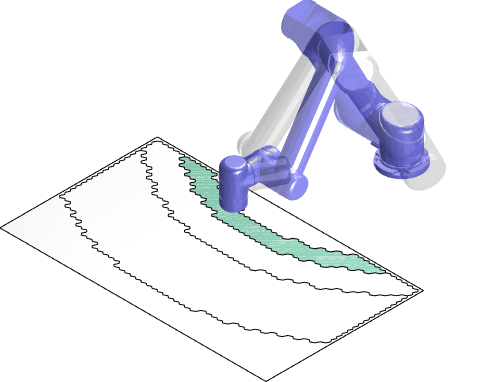
\includegraphics[width = 0.15\textwidth]{figures/square_example/simple_example_merged_545}
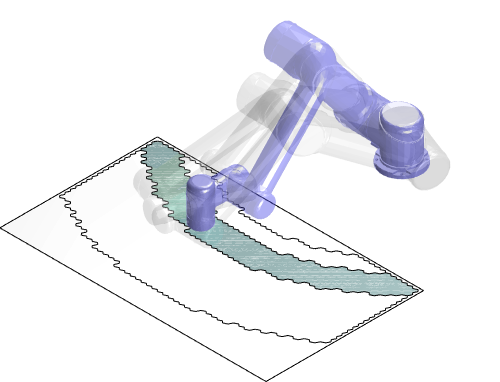
\includegraphics[width = 0.15\textwidth]{figures/square_example/simple_example_merged_551}
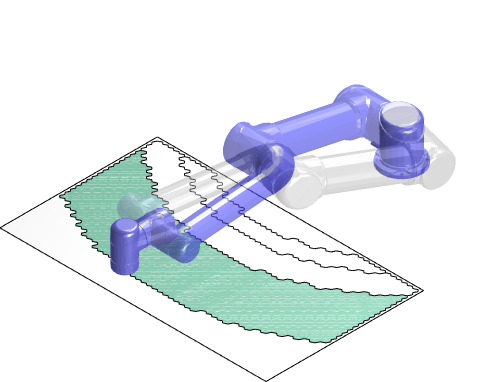
\includegraphics[width = 0.15\textwidth]{figures/square_example/simple_example_merged_565}
\caption{Illustration of different IK solutions covering the same points. Vivid configurations show one class of configuration: shoulder-right, wrist-unflipped, able to reach the vivid light cyan areas. Two additional configurations (shoulder-left/right, wrist-flipped) are also valid, shown shaded, although they can only cover the middle part of the reachable area, in shaded cyan. An unpainted surface section indicates unreachable by any configuration.}
\label{figsquare}
\end{figure}
\end{comment}

\begin{figure}[t]
\centering
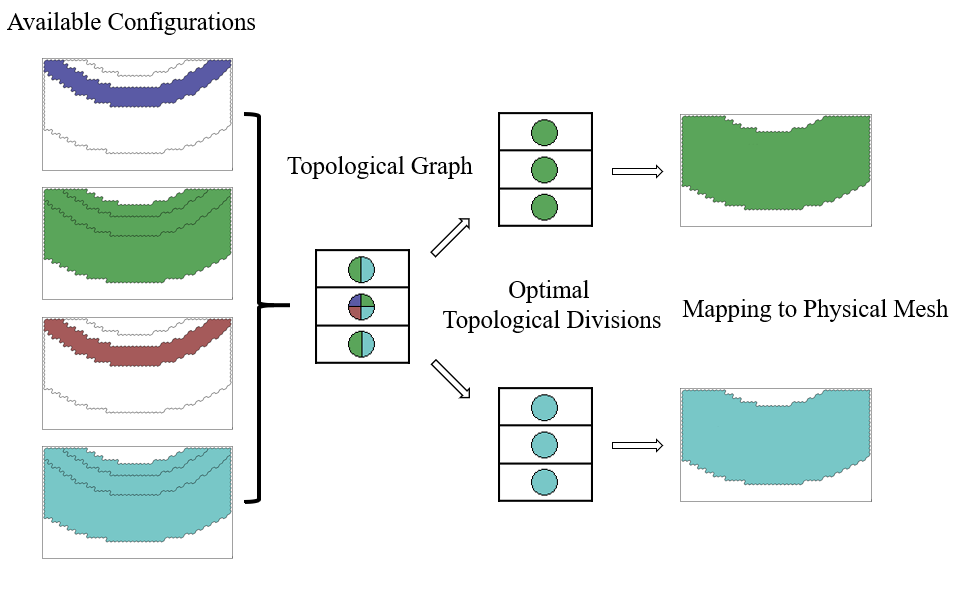
\includegraphics[width = 0.44\textwidth]{figures/other_figures/flowchart}
\caption{Proposed cellular decomposition solver the set-up in Fig.~\ref{fig:new_flowchart_2}. All configurations are divided into four disjoint (uniquely coloured) homogeneous sets, or cells, based on their joint-space continuities. The small circle filled-in with colour(s) represents all the possibilities to paint the corresponding area. A topological graph is created based on the distribution of the colours. Finally, in this example, two optimal options exist, both requiring zero lift-off.}
\label{fig:solver}
\end{figure}


\begin{comment}
\begin{figure}[t]
\centering
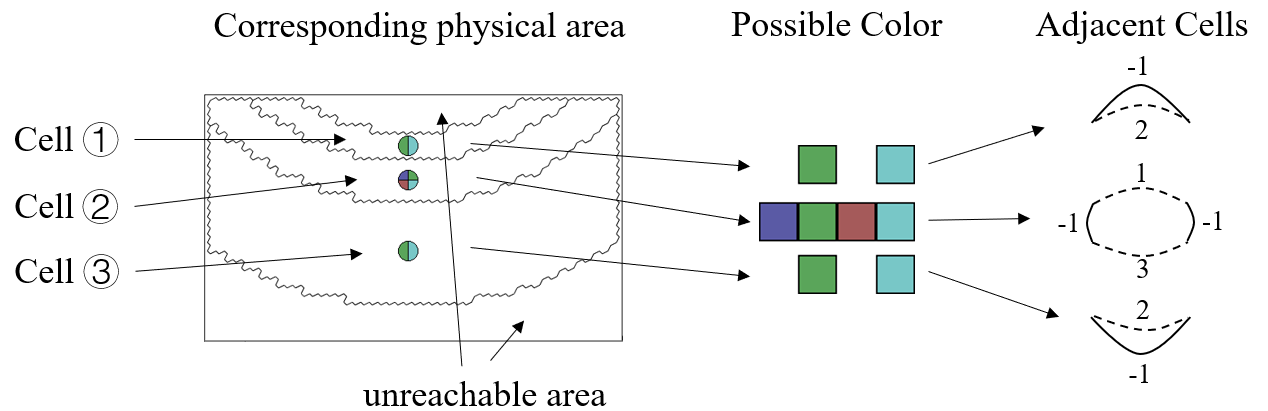
\includegraphics[width = 0.5\textwidth]{figures/other_figures/graphcreation_2}
\caption{
The elements of cells. All colours are indexed. Each cell corresponds to a connected area on the surface, and has a list of possible colours. A cell stores the index of its adjacet cell in order. % can you VERY briefly describe this for the example shown here, what numbers mean with respect to figure and the colours? e.g. for the middle cell, what is 2, 1, 3, using colours (blue, green, brown, cyan)
%\textcolor{blue}{
The index of the unreachable area is denoted by $-1$. Curves are used to indicate that the edge is topological, not physical. For example, cell 2 has four possible colours (blue, green, brown and cyan) and four edges which connect to cell 1, unreachable area, cell 3 and unreachable area in order.}
\label{figforcolor}
\end{figure} 
\end{comment}

\subsection{Independence from the Physical Coverage Path}
%An observation which simplifies the original problem is that the manipulator is omni-directional in the joint-space. A continuous joint-space path implicitly specify a continuous region in the joint-space in which we can find infinite many different coverage paths without lift-off. For example, in Fig.~\ref{fig1}, the ellipsoid in each set is coverable, whatever using a boustrophedon path in any direction, or using a spiral path starting from any boundary points. 
An observation which simplifies the original problem is that manipulators are locally omni-directional in the joint-space, and configurations corresponding to a segment of coverage path without lift-off have high dimensional continuity in the joint-space, regardless of their sequencing order. 
As a result, this work is inspired to consider only continuous regions in the joint-space and its corresponding reachable area in the workspace, instead of coverage paths in the task space, which is equivalent to a cellular decomposition problem in the workspace considering joint-space continuity. Under this equivalence, complete visiting of each cell is guaranteed with any arbitrary joint-space continuous path within, without discontinuities. 
Hence, once the cells are determined, the CPP problem within each cell 
is trivial, effectively transforming the design of the global coverage path in the traditional sense into a global cellular decomposition problem in joint-space, optimal in the number of lift-offs by incuring workspace partitions with minimum sets.
 
%\begin{color}{red}
%\subsection{Problem Modeling}\label{sectionmodelling}
%
%Without loss of generality, the input data is a triangular mesh, with all vertices and edges fully known. Then the normal of each vertex and all valid IK solutions to cover it are also known. 
%Since the manipulator is non-redundant, the number of IK solutions for each vertex is finite. 
%Although the mesh is a discretized data structure, we say two vertices are ``continuous'', if there is a list of edges of the mesh connecting them. And we say two configurations are ``continuous'' for the manipulator to reach, if the vertices are continuous, and the distance of these two configurations in the joint-space is near enough. The distance threshold for the continuity is easy to judge, since the manipulability constraint abandones the configurations which are close to the singularities, thus creates an apparent gap between disjoint sets. Typically, just the signs of the joint angles are enough to judge the continuity of two configurations. For example, it is easy to see that three vivid configurations in Fig.~\ref{figsquare} are continuous, and the greyed out configurations in a same figure are discontinuous pairwise. 
%
%First, we assign the colour of all configurations. Starting from an unassigned configuration, using a floodfill-like algorithm on the mesh, all configurations which are continuous with the chosed one are easy to find and are assigned with a same number, which is the index of the corresponding colour. After repeating the assignment process, all configurations have a colour, and the continuous configurations have a same colour. 
%Note that the IK solutions for the same vertex must have different colours. 
%So it is suitable to show the distribution of a colour through drawing them on the mesh. For example, Fig.~\ref{flowchart} shows the distribution of four colours of the example in Fig.~\ref{figsquare}.
%
%Second, we divide the mesh into several ``cells'', with each vertex belonging to a cell. The cell is a connected open region containing all vertices which are continuous and can be covered through same kinds of colours. 
%For the generation of a cell, we pick up an unassigned vertex, using a floodfill-like algorithm to find all continuous vertices which have same kinds of colours. 
%These vertices belongs to a single cell. In Fig.~\ref{flowchart}, we draw a small circle filled in with multiple colours to show the possible colours for a cell. After repeating the process, all vertices are assigned. 
%
%Third, after the creation of all cells, we say there is a topological edge between two cells, if there is a physical edge of the mesh which connects two vertices from different cells. 
%We may see the intersection of topological edges in the following figures, but note that they are formally drawed, since each edge connects only two vertices which are impossible to belong to three or more different cells. 
%In all, the structure of the topological graph is uniquely decided by the mesh. 
%
%Finally, the cell records the possible colours for covering the points and the index of its adjacet cells in order, see Fig.~\ref{figforcolor}. 
%Note that in practical application, since the area of the surface is finite, and each cell must have least size to keep the decomposition meaningful, the number of cells must be finite. 
%
%After creating the topological graph, the original problem is equivalent to painting all points with one of their available colours, ensuring the minimum pieces of colours. And for a fully-filled graph, the colour of a point uniquely specifies one of the valid IK solutions to cover it. 
%\end{color}

%\begin{color}{blue}
%\section{Problem Modeling with Symbols}
%\subsection{Problme Statement}
%Same as above.
%\subsection{Independence from the physical coverage path}
%Same as above.
\subsection{Modeling}
%First, we define some symbols. 
Let $\mathscr{C}$ be the set of all valid configurations and $M$ be the set of all reachable points on the surface. The pose of the EE is also denoted by $M$ since there is an one-to-one correspondence between the pose of the EE and the point on the surface, so we do not distinguish them. 

%Second, the \textit{colour} in Fig.~\ref{fig1} has significant meaning which deserves formal definition. 
%In mathematical terms, continuity of two configurations is an equivalence relation (reflexive, symmetric and transitive), 
%denoted by $\sim$. Then each element in the quotient set $\mathscr{C}/\sim$ corresponds to an unique class, chosen as a
% colour for easier visualisation. 
 
%Now we show the assignment of the colour in usual language. 
Given a configuration $p \in \mathscr{C}$ covering $m\in M$, following the joint-space continuity, there exist a neighbourhood $(p\in)U_p\subset \mathscr{C}$ that can be reached continuously (without lift-off) from $p$, covering a section of surface 
$(m\in )V_{m}\subset M$. This is illustrated in Fig.~\ref{fig:new_flowchart_2}, where the poses reached by the manipulator 
configuration depicted in vivid colour can be reached continuously - shown in vivid cyan. 
If any of them is chosen as $p$, then all of them are in $U_p$. 
Assuming there are some other unassigned configurations, i.e., $\mathscr{C}\backslash U_p\neq \varnothing$, 
choosing another  $p'\in \mathscr{C}\backslash U_p$ specifies another set $V_{m'}\subset M$ - e.g. the shaded 
configurations depicted in Fig.~\ref{fig:new_flowchart_2}. 
It is evident that $U_{p'} \cap U_{p} = \varnothing$. %Fixed <jvm> Tong pls make sure this is true, it is not evident to me, but I think I am missing something from notation. So long as it is to you, ok. % <ty> You are right, I made a mistake when changing the symbols. The sets in the joint-space is disjoint, not the workspace.  
On repeating this process, all configurations are assigned a colour. 
%\begin{color}{blue}
Let the number of configurations be infinite. Actually, each valid configuration implies an open neighbourhood of valid configurations covering an open region on the surface (defined sub-resolutionally if the input data is discretized, like a triangular mesh in our case). The family of all open regions on the surface implied by all valid configurations is an infinite open cover of the whole surface which, with physical meanning, must have boundary. Then, even if there are infinite many open regions in the family, the Heine-Borel theorem in mathematical analysis claims the existance of a subcover with finite open regions. The finiteness of a discretised input data is trivial because the number of configurations is also finite.
%\end{color}
As such, $\mathscr{C}$ is divided into a finite number of disjoint sets, denoted by a finite number of different colours. 
% where we omit the strict proof % <jvm> Tong, this looks prety critical to me! can you summarise your proof in any way? our key contibution is that the set is finite, but we don't prove!

The problem also exploits the concept of a \textit{cell} defined on the task-space, following the standard terminology 
of conventional cellular decomposition methods, but with the additional property of homogeneity. 
This is established on noticing that IK mapping from reachable points in the workspace to a single set of configurations is injective, since there is no non-singular path connecting two configurations whose EEs are at a same point (see graphic example in Fig.~\ref{fig1}). 
%The basic observation is that the IK mapping shown in Fig.~\ref{fig1} is injective in each branch. 
%The multiple IK solutions appear when the inverse trigonometric function returns multiple solutions. Corresponding to the physical meaning of the 5DOF manipulator, the multiple solutions of the elbow joint causes ``elbow-up/elbow-down'', etc.  
%Without strict proof, there exist a joint-angle leading to a singularity in between (``elbow-straight'' in this case). 
%%So there does not exist a joint-space path connecting two IK solutions of a same pose of EE without visiting a singularity. 
%For example, in each subfigure of Fig.~\ref{figsquare}, the greyed out configurations have the same pose of the EE with the vivid one, so they must be assigned with different colours. 
The injectivity of each branch of the IK is the motivation to map the property of joint-space continuity back on to the surface, thus the algorithm can be visualized by drawing colours on the surface to form cells belonging to the same configuration class (colour).  
Refering to the same square coverage example, Fig.~\ref{fig:solver} shows how $\mathscr{C}$ is divided into 4 disjoint sets. 
Since different IK solutions possess distinct colours, the available colours for points can be used to classify them. Let $\{c_i\}, i = 1, \cdots, n$ be all the colours used, then for two points $m_1, m_2\in M$ their sets of available colours are $c_{m_1} = \{c_{11}, \cdots, c_{1i}\}, c_{m_2} = \{c_{21}, \cdots, c_{2j}\}$. We then say that $m_1$ and $m_2$ belong to the same cell if and only if 
$$\left\{
\begin{aligned}
& m_1,m_2 \mbox{ are connected}\\ %\mbox{ and } 
& \{c_{11}, \cdots, c_{1i}\} = \{c_{21}, \cdots, c_{2j}\}
\end{aligned}
\right.
$$
Typically, for a triangular mesh surface as is our case, connectivity is provided by the edges of the mesh. Fig.~\ref{fig:solver} shows the creation of the cells. 


Finally, a topological graph is created, whose elements are cells. Each cell possesses an index, records the possible colours 
and the indices of its adjacet cells in order, as per the example in Fig.~\ref{fig:new_flowchart_2}. 
%Note that since the area of the surface is finite, and each cell must have the smallest size to keep the decomposition meaningful, the number of cells must be finite. % <jvm> Tong, is this sufficient? see my comment above re: finitness 
%\begin{color}{blue}
Since the number of colours is finite, the number of possible combinations of colours is also finite, which can be ordered as
$$\left\{
\begin{aligned}
&\{c_1\}, \cdots, \{c_n\}\\
&\{c_1, c_2\}, \cdots, \{c_1, c_n\}, \{c_2, c_3\}, \cdots, \{c_2, c_n\}, \cdots, \{c_{n-1}, c_n\}\\
&\cdots\ \mbox{(with all $i$-element combinations in the $i$-th row)}\\
&\{c_1, \cdots, c_n\}
\end{aligned}
\right.$$
For each combination of colours, the number of corresponding cells is finite, unless there are infinite many small cells with area zero, which is physically meaningless for the coverage task of the robots. In all, the number of cells must be finite. 
%\end{color}

After creating the topological graph, the cellular decomposition process is transformed into painting all points in a graph with 
one of their available colours.
The number of % pieces % <jvm> what is a `piece' ?? creating unnecesary new terms gets confussing, txt and figures should use the same terms (now they mostly do ...). I've given it a go, pls see if I am not mistaken
solutions to ``painting'' the full graph means the number of coverage path segments, where discontinuities are required in between, with the minimum(s) as best solution. Two valid solutions exist for the example in Fig.~\ref{fig:solver}. 
%So the optimal cellular decomposition problem is transformed to the painting problem ensuring the minimum pieces of colours. 
%For a fully-filled graph, the distribution of the colours specifies a cellular decomposition ensuring no lift-off required in each cell, and the choice from all IK solutions at all points are uniquely specified by the corresponding colour. So finally the problem is transformed to finding a colour scheme for the graph ensuring least number of pieces.
In summary, the proposed model of colouring a point in the surface to be covered means selecting a given IK solution for it, 
and the planning problem is thus transfered to designing a colour scheme for a topological configuration graph.

\begin{figure}[t]
\centering
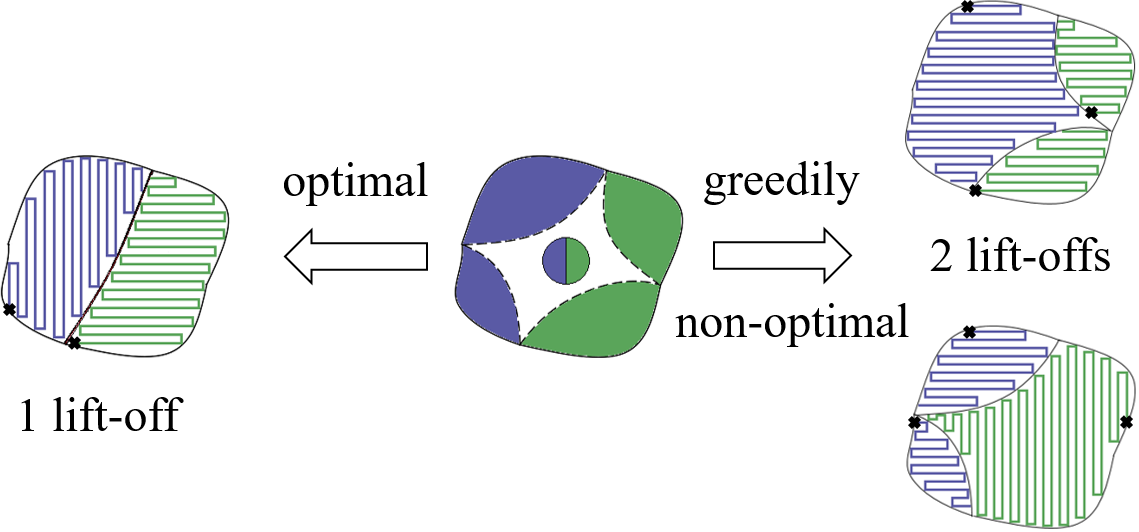
\includegraphics[width = 0.4\textwidth]{figures/other_figures/simple_3}
\caption{
In this example, only the middle cell still needs solving. From the two available colours, whatever the choice to fill the cell in its entirety incurs an extra, unnecessary lift-off. On the other hand, optimality is achieved when splitting the cell into two parts, 
with the two resulting sub-cells filled in with different colours, requiring only $1$ lift-off. 
}\label{figsimpleexample}
\end{figure}

\section{Enumerative Solver for Cellular Decomposition}
\label{sectionenumerativesolver}
The difficulty of solving the coloring problem is that, although points are gathered into homogeneous cells, 
they can be filled in with different colours, instead of only being seen as a whole and drawn with a single colour. 
The counter-example in Fig.~\ref{figsimpleexample} illustrates this phenomenon. 
By efficiently discarding equivalent cellular decompositions, it can be proven that the total number of different cellular 
decompositions is finite, thus all optimal solutions are finitely solvable. 

%Fixed <jvm> Tong, what are the dots ... to the left of figure? the case is complete, do we need them? I don't think so. If I'm wrong and we do, we need to explain what they are % <ty> Possibly unnecessary. The dots shows that it is only part of this equivalence, the other part should be applied to the other endpoint of the cutting path.
\begin{figure}[t]
\centering
\subfigure[Example shows that it is sufficient to consider cutting path which starts and end at the topological edge endpoints.]{
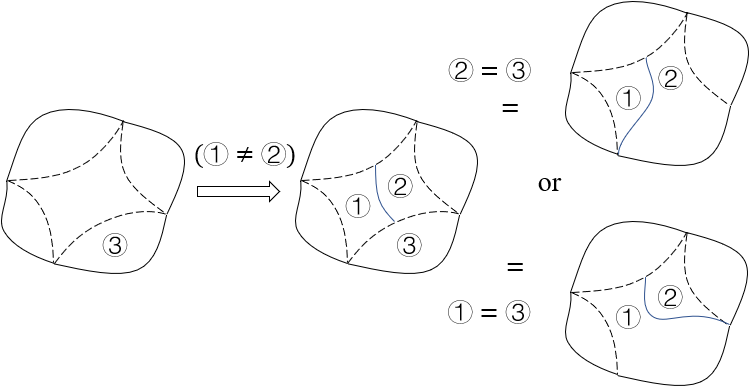
\includegraphics[width=0.4\textwidth]{figures/proof/equiv_cutting_path}}
%Fixed <jvm> does this example assume 1=2=3? I'm a bit confussed about this one ... see comment above % <ty> No problem here. It is impossible that 1=2, orelse there is no cutting path. 
\subfigure[Example shows that it is unnecessary to consider cutting paths that stretch across edges. 
]{
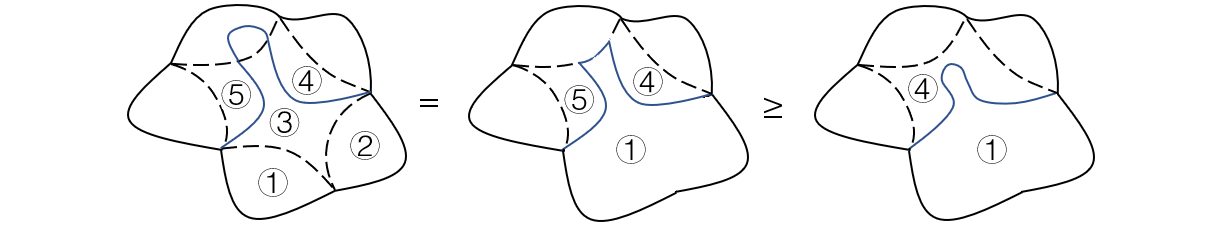
\includegraphics[width=0.48\textwidth]{figures/proof/equiv_cutting_path2_2}}
\subfigure[Example shows that intersecting cutting paths can be discarded.]{
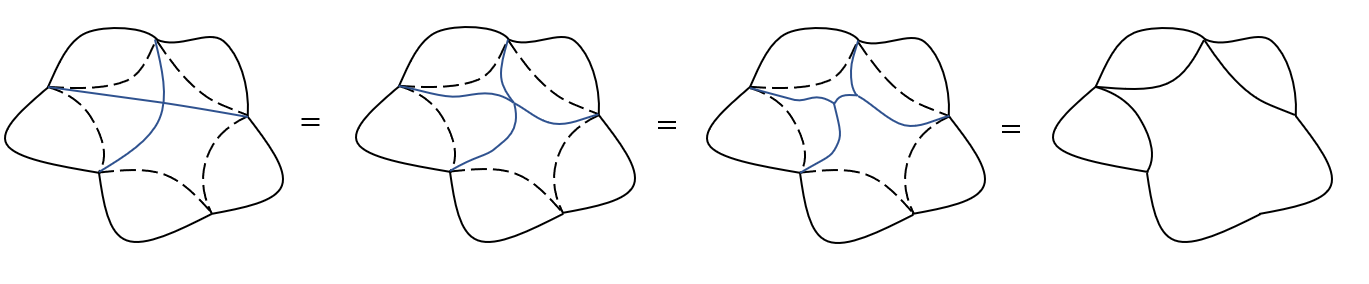
\includegraphics[width = 0.48\textwidth]{figures/proof/equiv_cutting_path3}}
\caption{Unnecessary or sub-optimal cell divisions cases can be safely discarded.}
\label{figproof}
\end{figure}

\subsection{Finiteness of Divisions}
\label{subsectionproof}
Since any path starting and ending at the boundary of a cell will divide the cell into two parts, there are infinite many physical solutions of dividing a cell into parts. However, there are only finite classes of them from a topological structure viewpoint 
because of the equivalence of physical divisions in the number of lift-offs. 

Fig.~\ref{figproof}(a) shows how cutting paths which start or end at a point other than an endpoint on an edge are unnecessary and can be pruned. Let a cutting path end at an arbitrary point of the edge connecting with cell 3. From the definition of a cutting path, it implicitly enforces cell 1 and cell 2 having different colours.  
If $1\neq 3$ and $2\neq 3$ the division is trivial. 
However, for the depicted cases when $1=3$ or $2=3$, any cutting paths that start at any endpoint of the edge are equivalent. Hence, for a complete solutoin it is sufficient to only consider cutting paths which start and end at the endpoint of an edge.  

Fig.~\ref{figproof}(b) shows how cutting paths which go across any edge are unnecessary. % <jvm> Tong some or all?? I take all % <ty> I'm not sure what do you mean. I guess you want to add the "any"? 
Let a cutting path go across an edge, then cell 4 and cell 5 are prevented from being coloured together which leads to non-optimality, since they are separated physically by the cutting path.
% <jvm> Tong, I don't understand what the case below is meant to represent, it seems a very specifc case out of many. 
% in pic I can see the case for the left 3 figures. But not the 4th, to the left. The case seem to be when 1=2=3, and 5=6, but there are many other, so I am confussed. Isn't enough to say the above, not below (commented out now), and remove fig to the left, to express the fact: no need to consider going over edges, full stop?? 
%This division enforces the constraint of colour that $3\neq 4, 3\neq 5, 3\neq 6$. However, it prevents cell 5 and cell 6 from being coloured together, because they are separated physically by the cell 3, which increases the cost and is thus not optimal. So we can directly discard the cutting paths which go across edges. 

Fig.~\ref{figproof}(c) shows that cutting paths need not go across each other. When two cutting paths intersect, 
%we can change the belonging of the path segment, 
the resulting cutting path segments can be continuously transformed back onto the existing topological edges, and can be safely diregarded.
%. So it is complete to discard the choices of cutting paths which have intersections. 

In conclusion, only cutting paths which start and end at the endpoint of topological edges and do not go across each other need to be considered when considering options for cell subdivision, making the total number of topological divisions finite. 
% and we just need to go through all possible divisions. 

\subsection{Solution to Simple Cells}
\label{sec:simple_cell}
The following kinds of cells offer simple cases that can be solved directly without further divisions:
\begin{enumerate}
\item Cells containing less than four edges. They cannot be divided further into several cells with less number of topological edges. Fig.~\ref{figeasycell3} enumerates all possible topological divisions for a three-edge cell, which constitutes the most complicated case for direct enumeration. Binary number are used to represent the edge connectivity, $1$ (connected), $0$ (disconnected). It is thus easy to see that there are at most $8$ situations that require consideration.
\item Cells with only one possible colour.
%\item Three-edge cells. Fig.~\ref{figeasycell3} enumerates all possible topological divisions for this case, which constitutes the most complicated case for direct enumeration. Binary number are used to represent the edge connectivity, $1$ (connected), $0$ (disconnected). It is thus easy to see that there are at most $8$ situations that require consideration.
\end{enumerate}

% <jvm> Tong, I don't really undertand the below, what other `further simplifications' can be possible, no more binary combinations ... But no time, so long as what we say below in caption is correct to you, leave it as is. If incorrect, or not needed, then maybe simplify caption by removing anything unnecessary?
\begin{figure}[t]
\centering
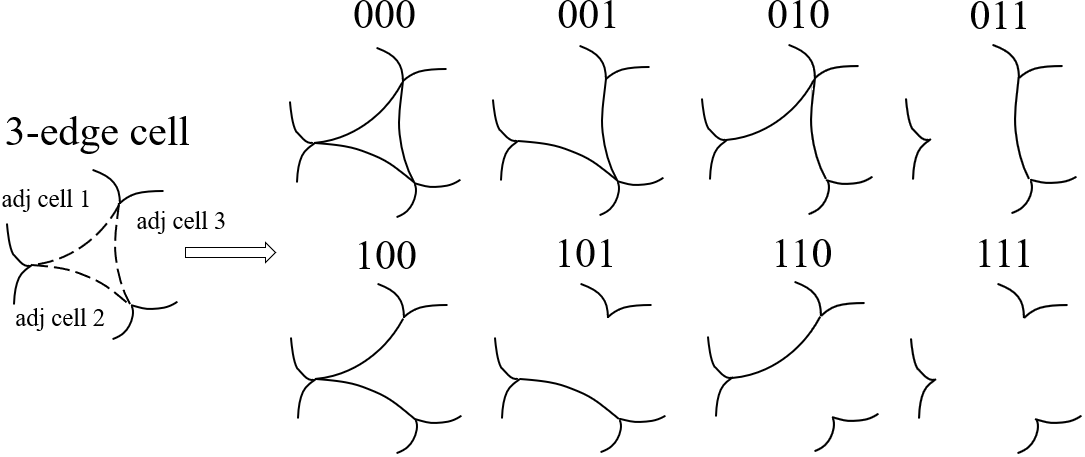
\includegraphics[width = 0.44\textwidth]{figures/other_figures/cell3}
\caption{Possible divisions of a 3-edge cell, as the most complex situation that need not further divisions. It can be observed how some of them are the same in terms of topological structure (e.g. $001, 010$ and $100$), 
or the division is impossible (e.g. $011$ is enforced, but cell 1 and 2 do not have the same colour), it is clearly already a finite problem, and the description of   further simplifications is omitted for clarity and space constraints.}
\label{figeasycell3}
\end{figure}


\subsection{Solution to Complex Cells}
The concept of using binary coding for a simple cell is extended to solve for an arbitrary $n$-edge cell, 
%length $n$ to represent the connectivity with $1$ for connection, $0$ for disconnection and 
with the addition of ``$\times$'' for a yet unspecified connectivity state that emanates from these more complex scenarios. 
For this binary combination, there are less than $2^n\times m$ branches for an $n$-edge cell with $m$ possible colours, so the problem remains finite. 
An example of solving for $n=4$ is shown in Fig.~\ref{figeasycell4}.
In this case, a continuous connected state ($1$s) implies that part of this cell must be painted with the same colour as that of the adjacent cells. % which the $1$s specify. 
On the other hand, a connectivity of $0$ indicates that the topological edge between the cell and the corresponding adjacent cell is maintained, and as such the colours must be different. 

\begin{figure}[t]
\centering
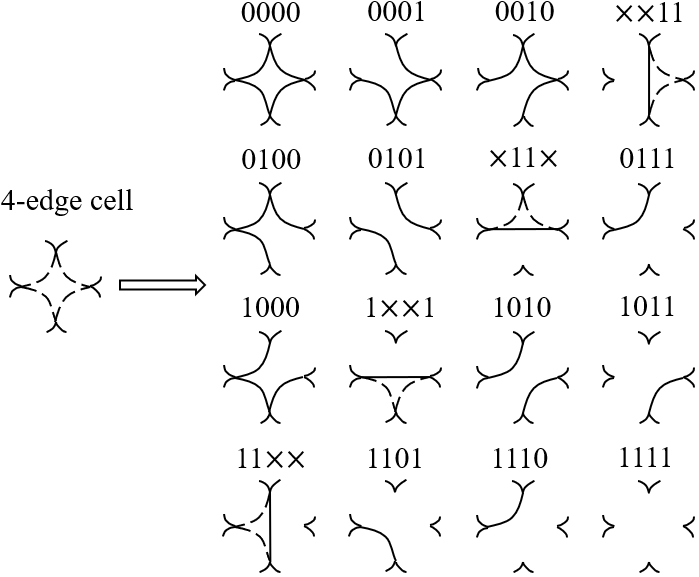
\includegraphics[width = 0.4\textwidth]{figures/other_figures/cell4}
\caption{The $2^4$ possible divisions of an 4-edge cell. For the cell which has more than 3 edges, the sub-cell may be created. In this figure, the connectivities that correspond to generating a sub-cell is $\times\times11, \times11\times, 1\times\times1, 11\times\times$. }\label{figeasycell4}
\end{figure}

The unspecified state $\times$ indicates a sub-cell will be generated. %Through specifying the position of $1$s, 
A more detail discussion about the distinction between $0$ and $\times$ is warranted:
%\subsection{Discussion of Creating Sub-Cells}
%\label{subsectiondiscussion}
when connectivity cases such as the following arise 
$$1\times\times1, 1\times\times\times1, \cdots$$
the cell is divided into smaller parts whose colours are enforced to be different, i.e. the cell needs further subdivision.
Refer for instance to cases $\times\times11, \times11\times, 1\times\times1, 11\times\times$ in Fig.~\ref{figeasycell4}. 
The original cell transforms into a new one with fewer edges, since some (two for a 4-edge cell) %Fixed <jvm> Tong, is this correct for 4-edge cell?
edges are replaced by a single one.  
We use the bracket notation $(\cdots)$ in the binary number of the original cell to represent the generation of sub-cells.
In recursively applying the same division for the applicable sub-cells, any $n$-edge cell can thus be continuously divided into 
a set of cells with fewer edges, suitable to then be solved enumeratively as described. % for the simple cell case in the preceding section.
% <jvm> Tong, where does this come from? see my next comment below
Since sub-cells are generated from an original one, there are extra constraints on its connectivity as specified by the previous division. 
%However, these constraints cannot change this problem into one with polynomial time solution, so we just give some examples among them: <jvm> Tong, this is a very loose statement, I feel unjustified. I don't see where the `polynomial' time solution comes from, we are only talking about being finite, not how long it takes. I don't see on anything stated thus far that the subdivision is 
As such, the following situations may arise:
\begin{enumerate}
\item Single $\times$ cannot form a sub-cell, because 
$$\cdots 1\times 1\cdots = \cdots 101\cdots \mbox{ or }\cdots 111\cdots$$
but both conditions of the right side are considered in other branches. This is why the $\times$ case does not apply 
to the 3-edge cell in Fig.~\ref{figeasycell3}.  
\item The $0$s can be freely moved outside the bracket, because of the equivalence 
$$\cdots\times1(0\times\cdots\times1)1\times\cdots = \cdots\times10(\times\cdots\times1)1\times\cdots$$ 
See Fig.~\ref{figconstraint}. 
The same is true for the right bracket based on the symmetry of the number list, since a cutting graph makes sense 
only when the inner two numbers at the boundary are $1$s. This is why there are no brackets in Fig.~\ref{figeasycell4}.
\item The new topological edge created by a cutting path must be retained as it is manually introduced as such 
(it will always be $0$, spliting a cell into different colours, it can not be be $1$ or $\times$).  
%Hence, for the entire problem, 
No extra possiblities appear after the division. 
\end{enumerate}

\begin{figure}[t]
\centering
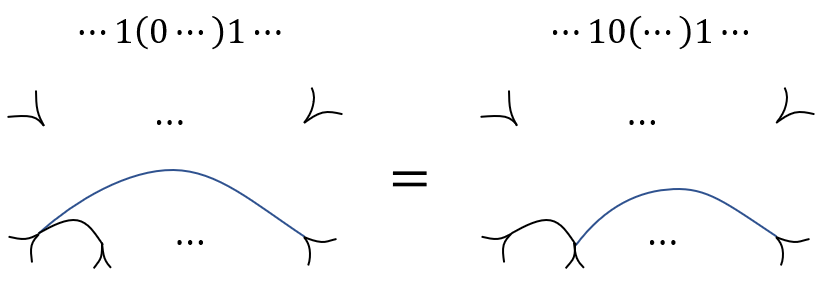
\includegraphics[width = 0.3\textwidth]{figures/proof/equiv_zero}
\caption{The equivalence of moving the unconnected $0$ state outside the bracket. Following this, in order to reduce the number of edges of a sub-cell, the equivalent sub-cell connectivity arrangement on the right is enforced.}
\label{figconstraint}
\end{figure} 


\section{Iterative Solver for Cellular Decomposition}
\label{sectioniterativesolver}
%\begin{color}{blue}
%The solving process is iteratively executed. In each iteration, the algorithm chooses an unsolved cell, finds its all possible solutions and creates a branch for each possible solution. In each branch, the chosed cell is filled in with the specified colour (so it will not change any more). 
%Then, in the next iteration, the algorithm chooses an unsolved branch, chooses an unsolved cell in it and does the same steps as before. 
%Finally, after iteratively solving, each branch becomes a valid scheme for coloring or returns with a contradiction. 
%The algorithm runs like the deepest-first-searching (DFS) algorithm so that the memory requirement is not high. 
%\end{color}

% <jvm> Tong I've done what I could on this section introduction (V, up to V-A), but I do not understand half of what is writtem here .... if you think it reads correctly DO NO CHANGE it. I don't, but that's ok at this point. 
%\subsection{Iteration Process}
With the enumerative solver as the basic building block, the graph can now be solved iteratively.
Starting from a fully-unpainted graph, an unsolved cell is arbitrarily chosed and enumeratively solved as 
described in Section~\ref{sectionenumerativesolver}. % <jvm> How is the initial one chosen, arbitrarily? randomly? can we very briefly describe the initial conditions for the iterative process?
Assuming a cell with $n$-edges with $m$ possible colours, there are \textit{at most} $2^n\times m$ possible divisions. A branch for each possible solution of the chosen cell is created, and in each branch the selected cell is filled in with the specfied colour (so it will not change any more). 
In the next iteration, an unsolved branch is selected, and an unsolved cell within it, and repeat the same steps.
 
Note that the constraints given by the solved adjacent cells significantly restrict the possible solutions, 
because the state of an edge resticts the connectivity of the cells on both sides. 
%After iterative execution, all branches reach a contradiction, % <jvm> Tong what does this mean here?? implicitly that is not a ``valid'' colour scheme, but I don't understand what that means ...
%or a valid coloring scheme. 
%\begin{color}{blue}
Through iterative execution, if there is a cell who cannot satisfy all constraints given by its solved adjacent cells, then the graph cannot be painted using the current state of the even partly-filled painting scheme, orelse a valid coloring scheme for the graph can be generated which uniquely specifies the configuration to polish each equivalent workspace point amongst the various valid IK solutions it may exhibit. 
%\end{color}

The search algorithm runs on a deepest-first-searching (DFS) format, so that the memory requirements are reduced. 
As an exhaustive search protocol, all optimal physical cellular decompositions must be homeomorphic to one of the resulting schemes.
%, with the position of the physical boundaries of the cells slightly different to the physical ones. % <jvm> Tong why? do we need to say this? omit otherwise, looks confusing and troublesome if review picks on this, I don't understand it
% <ty> do you mean the last part of the sentence or the whole sentence? I have at least removed the last part of the sentence. 

\subsection{Cost Calculation}
The physical meaning of the cost for a (partly filled) graph is the number of colour segments in the current portion of the graph, 
i.e. 1 colour equals cost = 1.
% (figuratively a single intial lift-off from a home position to cover the entire cell). 
The cost formulation is then described incrementally, whereby after a cell is solved
\begin{enumerate}
\item if its connectivity is all zero, then the cost will increase $1$ after freshly coloring this cell.
\item if its connectivity has only one $1$ connection to an already solved cell, then the cost will remain unchanged, since the cell colour can be filled homegeneously with the connected adjacent cell. 
\item if its connectivity has $i$ $1$s, there may exist multiple edges which connect the same adjacent cell, as per the illustration 
in Fig.~\ref{figcost}. In order to be consistent with the physical meaning of the cost, if these edges connect $j$ distinct solved cells, then the variation of cost is 
\begin{equation}
\Delta cost = 1-j
\label{eq:cost}
\end{equation}
\end{enumerate}

\begin{figure}[t]
\centering
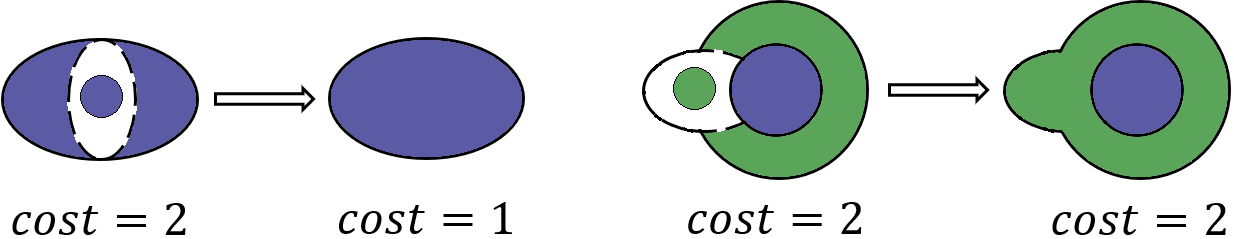
\includegraphics[width = 0.4\textwidth]{figures/proof/costcal}
\caption{Cost variation calculation. Left: the middle cell connects two distinct cells, so cost variation~(\ref{eq:cost}) is $1-2 = -1$. 
Right: two edges connect with the same adjacent cell, cost variation~(\ref{eq:cost}) is $1-1 = 0$.} % but not $1-2 = -1$.}
\label{figcost}
\end{figure}

% <jvm> Tong, add a table with the kinematic parameters of the UR5. Also add the size (length, diameter of buffet) of the polishing tool gimmick that you show on the real experiments
\begin{table}[tb]
\centering
\caption{UR5 Manipulator Kinematic Parameters}
\begin{tabular}{|>{ \bfseries }c | c | c | c | c |}
\hline
\normalfont{Joint i}   &     $\bm{\alpha_i}$ [rad]    &   $\bm{a_i}$  [m]    &    $\bm{\theta_i }$ [rad]   &    $\bm{d_i}$  [m]   \\
\hline
\hline
1 & $\pi/2$ & 0 & $\theta_1$ & 0.089 \\
\hline
2 & 0 & $-0.425$ & $\theta_2$ & 0 \\
\hline
3 & 0 & $-0.39225$ & $\theta_3$ & 0 \\
\hline
4 & $\pi/2$ & $0$ & $\theta_4$ & 0.11 \\
\hline
5 & $-\pi/2$ & 0 & $\theta_5$ & 0.09 \\
\hline
EE & $0$ & 0 & - & 0.32\\
\hline 
\end{tabular}

\label{table:ur5_kinematics}
\end{table}


\section{Experimental Results}
\label{sectionexperiment}
The proposed algorithm performs non-repetitive coverage task using non-redundant manipulators of any dimension. 
Simulation and experimental examples emulating a polishing task on an object's surface are presented in this section implemented using a typical 6 DoF manipulator, 
a Universal Robots UR5. The kinematics of the 6 DoF manipulator are collected in Table~\ref{table:ur5_kinematics}.
For such endeavour, the (commonplace) final revolute joint of the manipulator is unnecessary given the rotating nature of the polishing tool itself. This is indeed the case for the UR5,  
and simulations and real evaluation have thus been undertaken where the last link has been locked.
%Whilst the proposed work can be exploited to find the ideal placement of a manipulator to fully cover the surface of an object,  it is not the objective and the experimental results are thus set to cover all reachable points from the arbitrary location in the workspace where the manipulator has been located. 

% <jvm> Tong see further below
%First, we discuss the proposed algorithm using behind other cellular decompositions, from which the proposed algorithm can be seen as a tool for the evaluation of other cellular decomposition algorithms. 
In the first simulated experiment in Section~\ref{sec:wok_sim_examples} a hemispherical object is polished at different poses in the workplace: one arbitrarily set, and the other precisely crafted to be fully reachable with the least number of lift-offs, which shows the ability of the proposed algorithm to also become a workspace design metric for evaluating the quality of the object placement to be inspected. 
The second simulated experiment in Section~~\ref{sec:cyl_sim_examples} shows how the proposed algorithm can directly influence the choice of configurations 
to avoid non-optimal configurations that invariably lead to unnecessary lift-offs altogether.
Additional examples with objects of arbitrary shape are collected in Section~\ref{sec:other_sim_examples}.
Finally Section~\ref{sec:real_examples} depicts real-world experiments with a UR5 manipulator polishing a wok 
%following a manually generated physical coverage path 
in free space, and under the presence of obstacles, to proves the applicablity of the proposed algorithm in real settings. 


In the results shown hereafter 
%Unless otherwise stated, 
the environment contains the manipulator, the object being polished, and where applicable a ground plane and additional obstacles. 
%Furthermore, as highlighed in Section~\ref{subsectionproof}, it is worth noting that there are infinite physical cutting paths to decompose cells that result in the same number of lift-offs, 
Moreover, figures shown in this section are representative examples of arbitrary paths derived within the cells attained following the proposed optimal coverage solution. 

\begin{comment}
%Fixed <jvm> Tong This has nothing to do with ``experiments''. We could add before, but I don't see the point. what is really required in experiments is a comparison with one of the other cellular decomposition methods discussed in state-of-the-art, and see that your proposal ends up with less lift-off comparing the numbers, nor `prove' that it will be less. Most certainly not on the experimental results section of a paper!!! I've commented out, too late to change now. For future, you would want to compare the number of lift-off resulting from another cellular decomposition methos for examples in Fig 11, 12, 13, etc
% <ty> Actually it follows from Yue Wang's advice that we provide not only an "algorithm" but a "tool". We don't require the user to make trade-offs between our method and other methods.

\subsection{Calculating least number of discontinuities for other methods}
Since all cellular decompositions divide the whole reachable region into parts, implicitly imply discontinuities between cells. Then, the original problem can be solved through finding coverage path in each cell, and the result path is the concatenation of the path segments in each cell using paths where the EE is lifted off. Let a cellular decomposition methods divides the surface into $n$ parts, then $n-1$ lift-offs are required. However, notice that tracking the coverage path in each cell still requires lift-off, denoted by $p_i$. Then the least number of lift-offs a given cellular decomposition is 
$$n-1 + \sum\limits_{i = 1}^n p_i$$ 
where $p_i$ can be calculated through using the proposed algorithm in the $i-$th cell. 

To show the optimality of the proposed algorithm, we apply it to the cellular decomposition created by itself. Since each cell is guaranteed polishable with no lift-off, $p_i = 0, \forall i$. Moreover, the number $n$ is optimal since we use haustive seraching strategy. Hence, the proposed algorithm certainly outperforms other methods in the sense of the number of lift-offs. 
\end{comment}


\begin{figure}[t]
\centering
\subfigure[]{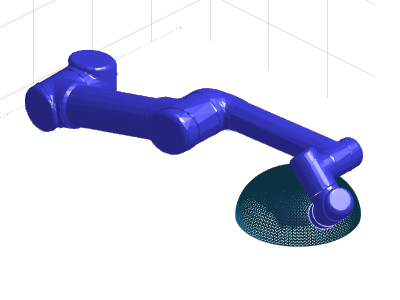
\includegraphics[width = 0.10\textwidth]{figures/simu_exp/exp_semi_ellipsoid/casual_demo}}
\subfigure[]{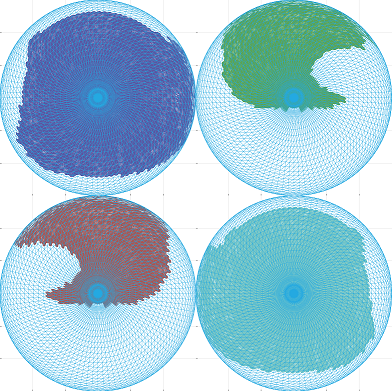
\includegraphics[width = 0.10\textwidth]{figures/simu_exp/exp_semi_ellipsoid/casual_comb}}
\subfigure[]{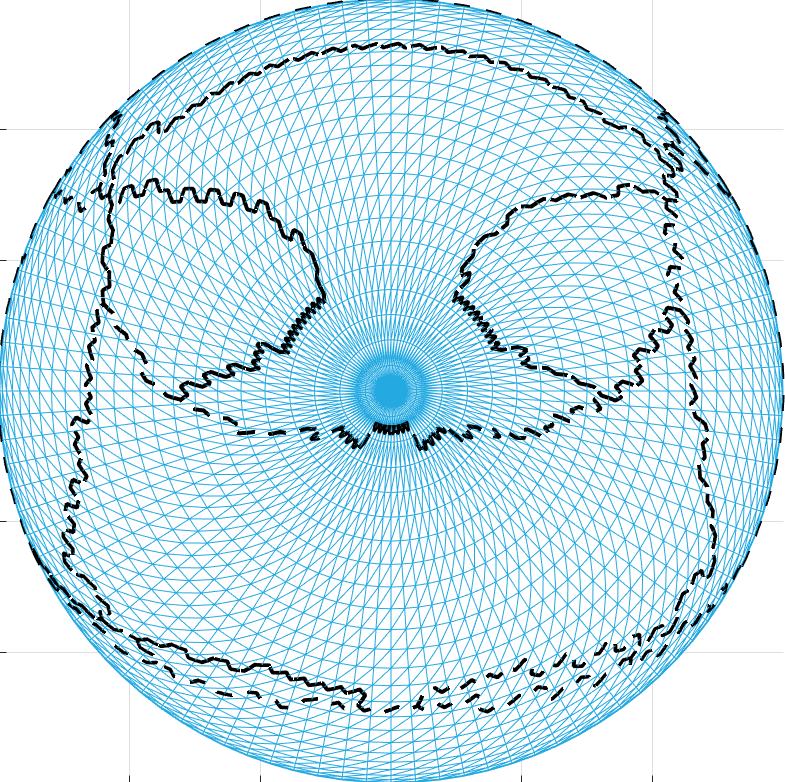
\includegraphics[width = 0.10\textwidth]{figures/simu_exp/exp_semi_ellipsoid/casual_init_graph}}
\subfigure[]{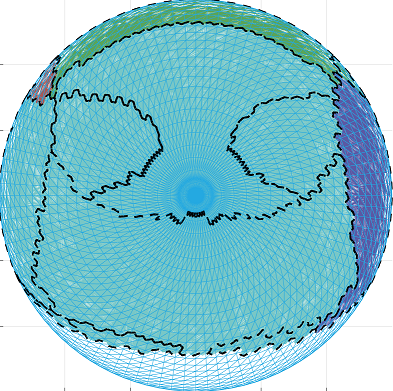
\includegraphics[width = 0.10\textwidth]{figures/simu_exp/exp_semi_ellipsoid/casual_result_graph}}
\caption{(a) Hemispherical object arbitrarily placed in the workspace. 
(b) Coloured cells of four valid configuration, chosen by the optimal solution shown in (d). %Fixed  <jvm> Tong can we say `the' four valid configurations coloured cells, indicating these are all the possible configurations? looks like it, but I'm not sure
% <ty> It is a coincidence. some symmetric configurations have same function. So I suggest we don't change. 
(c) Topological graph. (d) One optimal solution requiring 3 lift-offs 
(note how the manipulator cannot fully cover the farthest part of the mesh - the bottom area in the optimal solution, unpainted). 
}\label{figflatwise}
\end{figure}
\begin{figure}[t]
\centering
\subfigure[]{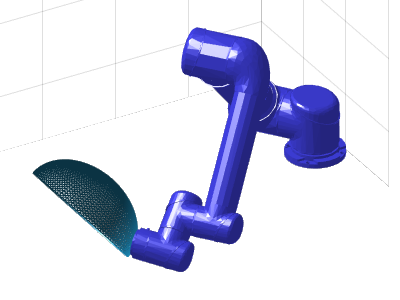
\includegraphics[width = 0.1\textwidth]{figures/simu_exp/exp_semi_ellipsoid/design_demo}}
\subfigure[]{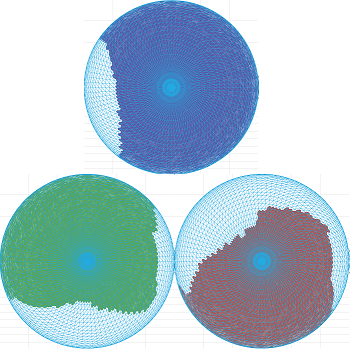
\includegraphics[width = 0.1\textwidth]{figures/simu_exp/exp_semi_ellipsoid/design_comb}}
\subfigure[]{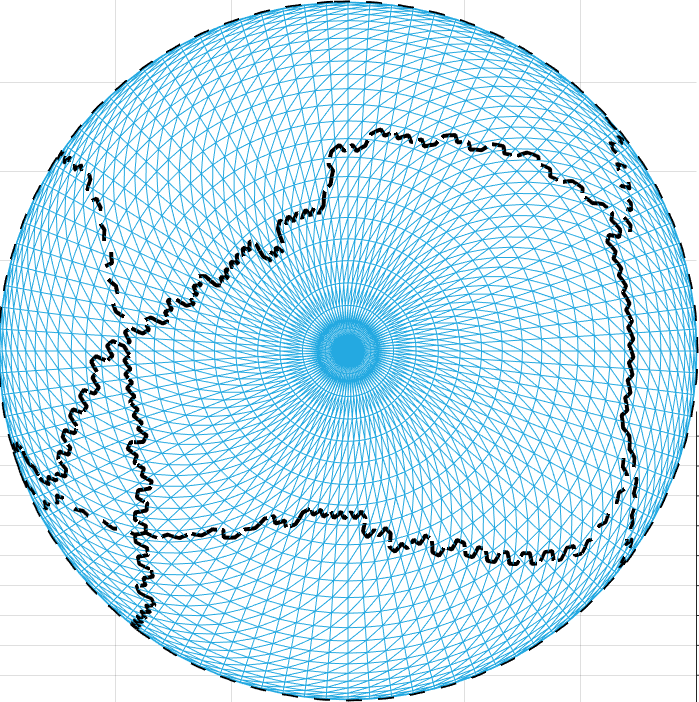
\includegraphics[width = 0.1\textwidth]{figures/simu_exp/exp_semi_ellipsoid/design_init_graph}}
\subfigure[]{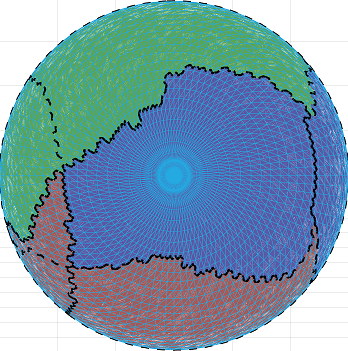
\includegraphics[width = 0.1\textwidth]{figures/simu_exp/exp_semi_ellipsoid/design_result_graph}}
\caption{(a) Hemispherical object placed obliquely in the workspace to achieve full coverage. 
(b) Coloured cells of three valid configuration, chosen by the optimal solution shown in (d). %Fixed <jvm> Tong as above? %<ty> as above.
(c) Topological graph. (d) One optimal solution requiring only 2 lift-offs and achieving fully coverage, with the object fully painted over). 
}\label{figsloped}
\end{figure}


\subsection{Hemispherical Object (Object Placement Criterion)}
\label{sec:wok_sim_examples}
%In this simulation experiment, through the polishing task of a hemisphere shape object, we show that the number of lift-offs provided by our algorithm can evaluate the quality of the placement of the object (or the manipulator). 
A wok-like round mesh is used for this experiment. Results are collected in Fig.~\ref{figflatwise} and Fig.~\ref{figsloped}. 
In the former, the object is arbitrarily placed with respect to the robot, as would be the case, for instance, on an automated production line with unsorted objects are fed via a conveyor belt. A CPP is designed following the proposed scheme. With no criterion for the placement, the algorithm shows that such an object placement requires at least $3$ lift-offs to inspect the reachable area, yet fails in attaining full coverage (the farthest area, shown at the bottom of the mesh, is out-of-bounds).
% which is equivalent to at least $4$ lift-offs. Fixed <jvm> Tong why do you say this? it is out-of-reach, no matter how many lift-offs?? <ty> Yes. I thought we can say "moving the object to another poses and requires an extra lift-off". It is also good for omitting them. 
Fig.~\ref{figsloped} illustrates the case where the proposed coverage strategy reveals a suitable pose for the object so that not only the required least number of lift-offs is decreased to $2$ when compared to the arbitrary placement, 
but the manipulator can fully cover the surface.
%Hence, the required number of lift-offs guides the user to try different poses of the object (or the manipulator) to have better performance on coverage. 

\begin{figure}[t]
\centering
\subfigure[]{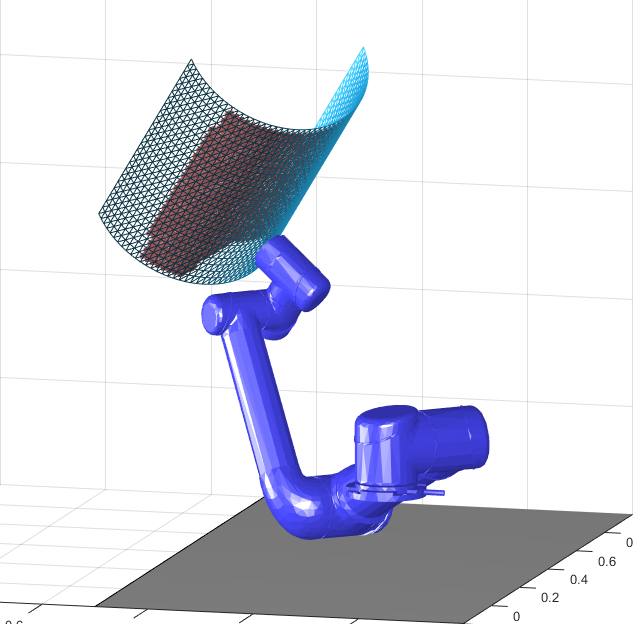
\includegraphics[width = 0.13\textwidth]{figures/simu_exp/exp_pipe/demo}} \qquad
\subfigure[]{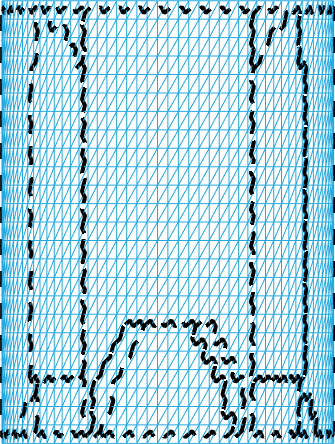
\includegraphics[width = 0.09\textwidth]{figures/simu_exp/exp_pipe/init_graph}} \qquad
\subfigure[]{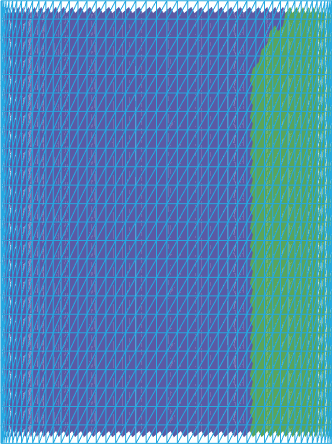
\includegraphics[width = 0.09\textwidth]{figures/simu_exp/exp_pipe/result_graph}}
\caption{(a) A cylindrical half-pipe object. (b) The topological graph. (c) One optimal solution which requires only 1 lift-off.}
\label{fighalfpipe}
\end{figure}

\begin{figure}[tb]
\centering
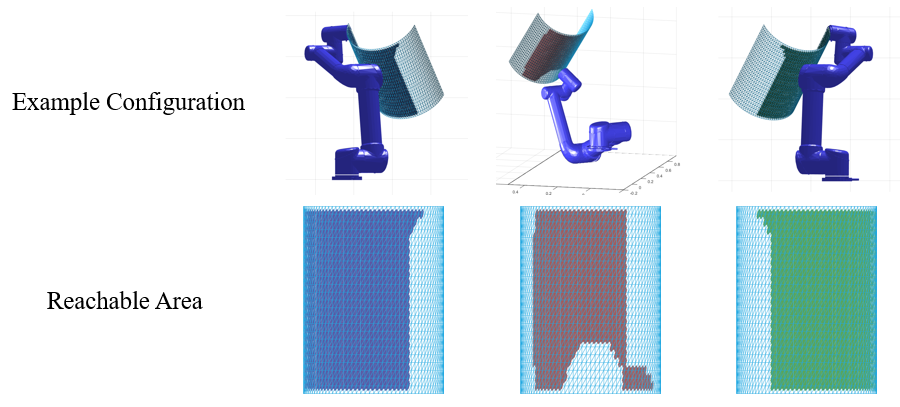
\includegraphics[width = 0.4\textwidth]{figures/simu_exp/exp_pipe/three_example_pose}
\caption{Example with three different configurations and their reachable area. Once any configuration belonging to the middle cell is chosen to cover the surface, sooner or later it will have to change to the left and right cells to finish the full coverage of the surface, thus incurring a wasteful lift-off.}
\label{figthreeexamplepose}
\end{figure}

\subsection{Cylindrical Object (Pruning of Suboptimal Configurations)}
\label{sec:cyl_sim_examples}
Polishing of a half-pipe is employed in this simulation to demonstrate how the proposed algorithm can identify and bypass unnecessary configurations leading to ``traps'' that cause CPPs with extra lift-offs. 

The pipe is placed obliquely to achieve full coverage. Surface normals vary along the arc length of the cylinder 
over $\pi$ radians, which cause increased difficulty in kinematic terms for the manipulator 
to sustain the desired polishing operation. 
The topological graph and optimal solution are shown in Fig.~\ref{fighalfpipe}, where it can be seen that the full coverage task requires only $1$ lift-off. 
However, there are many valid configurations which lead to non-optimality. 
%because they just cover some points which have many IK solutions but break the connectivity of the uncovered region. 
See Fig.~\ref{figthreeexamplepose} for an example of such ``trap'' configurations. 
The configurations on the left and right are the ones finally chosen by one of the optimal solutions shown in Fig.~\ref{fighalfpipe}. 
However, while the configuration in the middle can cover a large area without lift-offs, and would therefore be equally likely to be chosen if the IK solutions were to be selected randomly or in a greedy fashion, it cannot reach the corners of the mesh (eventually covered by the other two configurations). Hence, should any configuration from the middle be selected to trace 
the object, after coverage of (a section) of the middle part of the pipe, sooner or later the CPP will have to undertake one unnecessary lift-off for full coverage inspection, leading to non-optimality when compared to the case shown in Fig.~\ref{fighalfpipe}. The proposed algorithm will provide all optimal solutions, with none of them using the middle coloured cell.



\begin{table*}[t]
\centering
\caption{Coverage Planners Comparison}
%\begin{tabular}{|c|c|c|c|c|c|c|c|c|}
%\hline
% & \multicolumn{2}{c|}{\textbf{Ours} (Boust.)} & \multicolumn{2}{c|}{\textbf{Ours} (Spiral.)} & 
%\multicolumn{2}{c|}{Spiral (x10)} & \multicolumn{2}{c|}{Boust. (x10)}\\
%\cline{2-9}
%& Lift-offs & Time&Lift-offs & Time&Lift-offs & Time&Lift-offs & Time\\
%\hline
%Hemisphere & 1 & &1 & &36.6 & & &\\
%\hline
%Cylinder & 1 & & 1 & & & & &\\
%\hline
%Vase & 1& & 1 & & & & &\\
%\hline
%L-Pipeline & & & & & & & &\\
%\hline
%Klein bottle & 3 & & 3 & & & & &\\
%\hline
%\end{tabular}
\begin{tabular}{|c|c|c|c|c|c|c|}
\hline
 & \multicolumn{2}{c|}{\textbf{Ours}(with Boust.)} & \multicolumn{2}{c|}{Pure Spiral (10 average)} & \multicolumn{2}{c|}{Pure Boust. (10 average)}\\
\cline{2-7}
& Lift-offs & Time&Lift-offs & Time&Lift-offs & Time\\
\hline
\hline
Hemisphere & 2 & 3175.9 &35.6 &1503.3 &3.5 &3941.3\\
\hline
Half pipe & 1 &840.75&33.2&1055.8&3.3&768.4\\
\hline
Vase & 1&1101.47&31.4&2425.2&2.8&902.76\\
\hline
Full pipe&3&924.47&86.4&3365&59.8&3608.8\\
\hline
\end{tabular}
\label{table:comparative_results}
\end{table*}


\subsection{Arbitrary Shape Objects and Comparative Analysis}
\label{sec:other_sim_examples}
Further simulation tests are also shown on Fig.~\ref{fig:vase_sim} and~\ref{fig:fullpipe_sim}, where the robot arm was 
made to fully trace the surface of objects of arbitrary shape with the proposed algorithm. 
In the former instance a vase is considered, whereas a full-pipe is consider in the latter. 

To better appreciate the effectiveness of the proposed scheme, a comparative analysis is provided to contrast key relevant metrics with a standard geometric planner. Number of lift-offs  and total time taken to complete the coverage task were collected and are shown in Table~\ref{table:comparative_results}. For a fair evaluation, the pure spiral and boustrophedon planners are assumed to know in advance the non-reachable points on the surface, so they can be disregarded. Given the reliance of these planners on the starting point of the paths, the results are averaged over 10 runs where random starting points are observed. A variety of objects are studied, beyond those singled out in the previous sections -  individual detailed solutions for each case are omited given space limitations. It is clearly apparent how the optimal solution suggested by the proposed CPP planner markedly outperforms any of the other planners for the coverage task.


\begin{figure}[t]
\centering
\subfigure[]{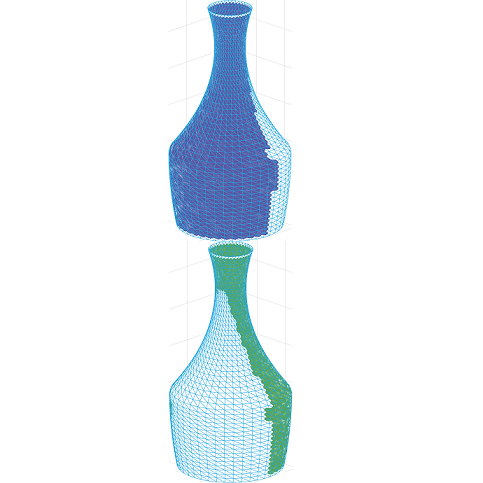
\includegraphics[width = 0.11\textwidth]{figures/simu_exp/exp_vase/color_comb}}
\subfigure[]{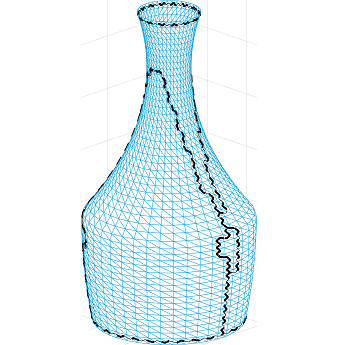
\includegraphics[width = 0.11\textwidth]{figures/simu_exp/exp_vase/init_graph}}
\subfigure[]{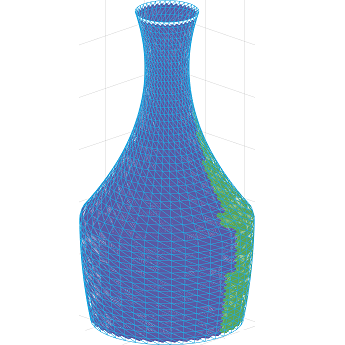
\includegraphics[width = 0.11\textwidth]{figures/simu_exp/exp_vase/result_graph}}
\subfigure[]{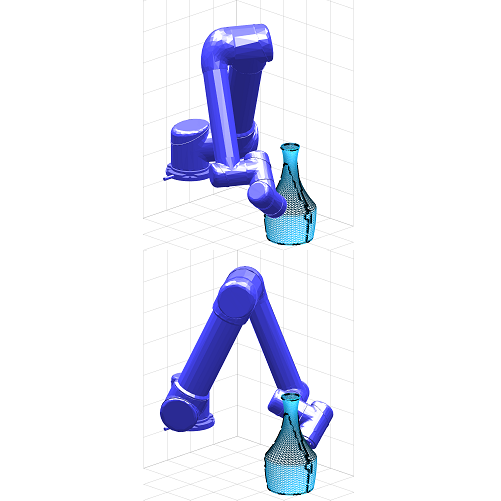
\includegraphics[width = 0.11\textwidth]{figures/simu_exp/exp_vase/demo_comb}}
\caption{Vase example. (a) Reachable coloured cells of two valid configurations, chosen by the optimal solution shown in (c). 
(b) Topological graph. (c) One of the optimal solutions requiring only 1 lift-off. 
The cutting path is arbitrary. (d)  Examples of poses in the two types of configurations.}
\label{fig:vase_sim}
\end{figure}

\begin{figure}[t]
\centering
\subfigure[]{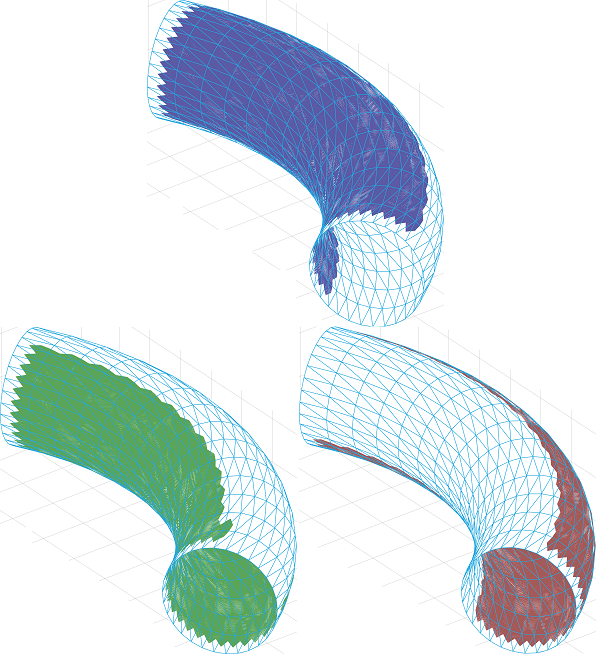
\includegraphics[width = 0.11\textwidth]{figures/simu_exp/exp_fullpipe/color_comb}}
\subfigure[]{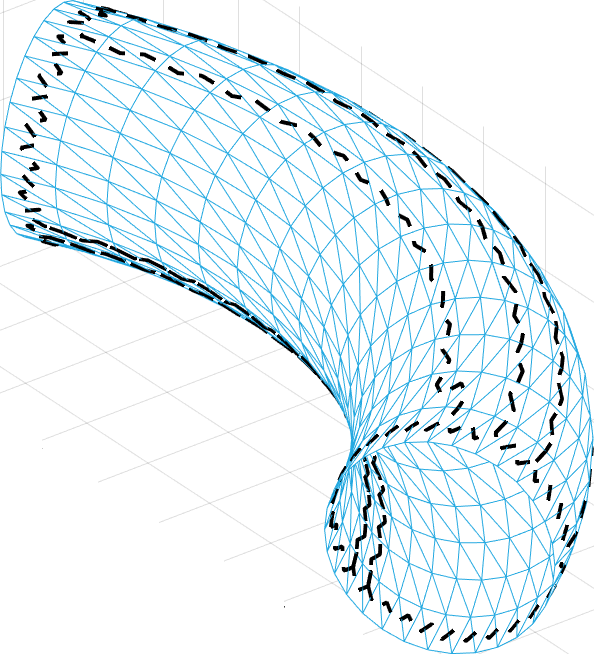
\includegraphics[width = 0.11\textwidth]{figures/simu_exp/exp_fullpipe/init_graph}}
\subfigure[]{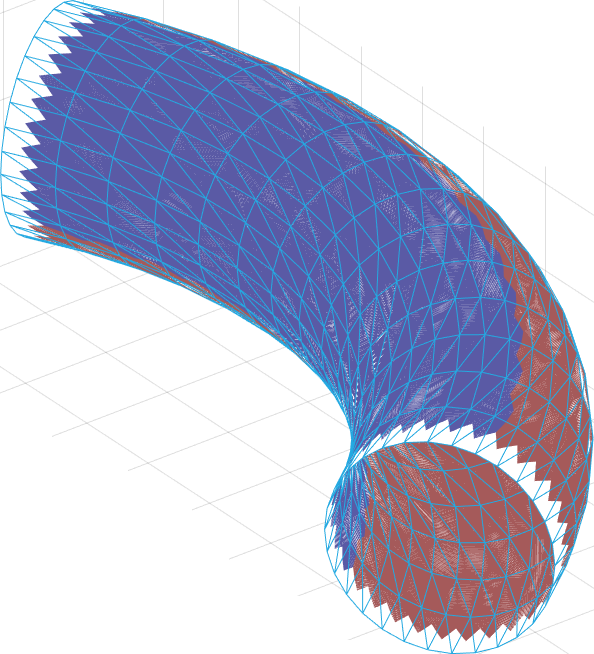
\includegraphics[width = 0.11\textwidth]{figures/simu_exp/exp_fullpipe/result_graph}}
\subfigure[]{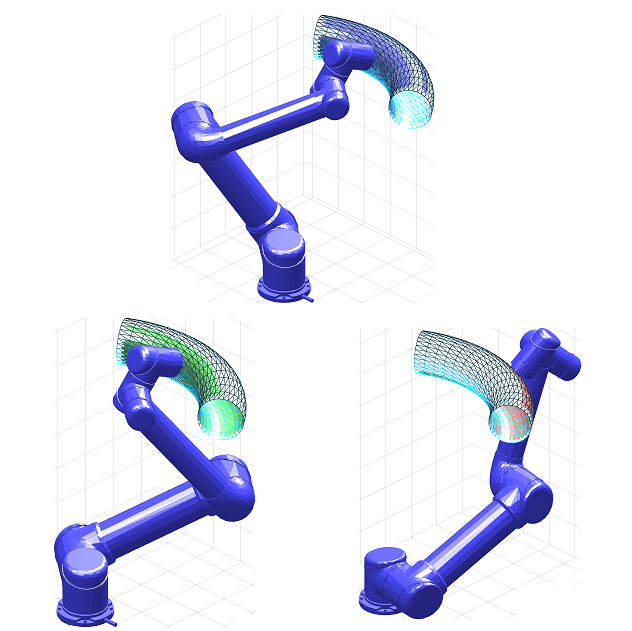
\includegraphics[width = 0.11\textwidth]{figures/simu_exp/exp_fullpipe/demo_comb}}
\caption{Full-pipe example. (a) Reachable coloured cells of two valid configurations, chosen by the optimal solution shown in (c). 
(b) Topological graph. (c) One of the optimal solutions requiring only 1 lift-off. 
The cutting path is arbitrary. (d)  Examples of poses in the four types of configurations.}
\label{fig:fullpipe_sim}
\end{figure}


% add comparison on its own section? TBC once I see results
%\subsection{Discussion of Results}
%\label{sec:comparison}


\subsection{Real World Experiments in the Presence of Obstacles}
\label{sec:real_examples}
A Universal Robots UR5 manipulator is employed for real experimentation to polish the outer surface of a wok to show a physical coverage path generated based on 
the proposed cellular decomposition method. The actual physical coverage path uses a simple back-and-forth motion (boustrophedon) within the resulting cells, 
with a lift-off concatenation between paths segments belonging to different cells. 
The reader is  referred to the associated  video\textsuperscript{\ref{video}} for the full demonstration. % are manually demonstrated. 
As discussed, the manipulator operates in a 5 DoF configuration. %, which is non-redundant. 
Since hybrid position/force control~\cite{solanes2019robust} is beyond the scope of this work, contact is restricted to position control. 

\begin{figure}[t]
\centering
\subfigure[]{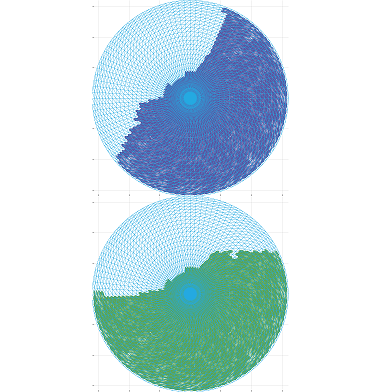
\includegraphics[width = 0.14\textwidth]{figures/real_world_exp/no_obstacle_comb}}
\subfigure[]{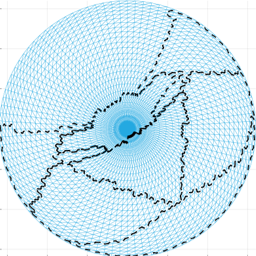
\includegraphics[width = 0.14\textwidth]{figures/real_world_exp/no_obstacle_initial_graph}}
\subfigure[]{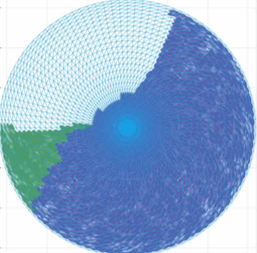
\includegraphics[width = 0.14\textwidth]{figures/real_world_exp/no_obstacle_result_graph}}
\subfigure[]{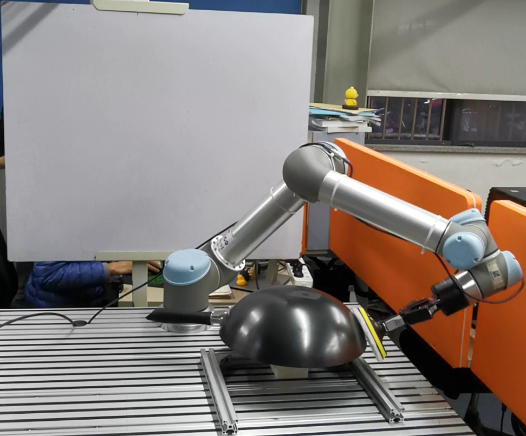
\includegraphics[width = 0.14\textwidth]{figures/real_world_exp/no_obstacle_demo_1}\label{fig:real_free_extreme1}} \hfil
\subfigure[]{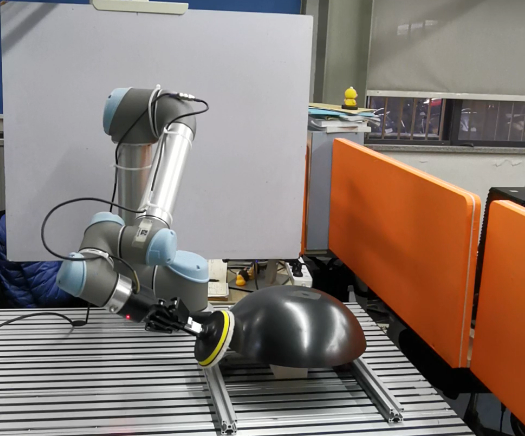
\includegraphics[width = 0.14\textwidth]{figures/real_world_exp/no_obstacle_demo_2}\label{fig:real_free_extreme2}}
\caption{(a) Reachable coloured cells of two valid configurations, chosen by the optimal solution shown in (c). 
(b) Topological graph. (c) One of the optimal solutions requiring only 1 lift-off. 
The cutting path is arbitrary. (d),(e) Examples of extreme poses in the two types of configurations.}
\label{fig:realworld_no_obs}
\end{figure}


Fig.~\ref{fig:realworld_no_obs} illustrates the results. Given the location of the wok, it can be seen how the nearest %and farthest 
part of the wok is unreachable. 
As can be observed in Fig.~\ref{fig:real_free_extreme1} and~\ref{fig:real_free_extreme2}, 
the manipulator must keep its wrist configured in the ``above'' the fore-arm configuration in order to 
avoid collisions, which leads to the two shoulder-left and shoulder-right configuration solutions. 
The total number of lift-offs is $1$. 
%Since each colour covers some points which only have one possible colour, the solution is definitely optimal. 
Note that any division keeping the resulting cell connectivity guarantees full (reachable) coverage and is optimal in the minimum number of lift-offs, so the cutting path dividing the final cell is arbitrary. 
% so we may just divide the surface through the middle. 

A more interesting example arises when the motion of the manipulator is obstructed by the cylindrical obstacle 
depicted in Fig.~\ref{fig:realworld_obstacle}. Since the obstacle may collide with the upper-arm, fore-arm or the EE, 
and the wrist may collide with the fore-arm, %Fixed <jvm> Tong or upper-arm? read above example, should be the same? same in figure caption, pls double check
% <ty> fore-arm. The wrist joint is not purly spherical, so it will hit fore-arm when folded. 
the resulting colour cell decomposition and the topological graphs is more complex. As such, to avoid collisions, 
the least number of lift-offs is shown to be 2. 
%Similarly, each colour covers some points which only have one possible colour, so the solution is also optimal. 

%Fixed <jvm> Tong not sure why these figs are different to the ones on your 2Jan20 version, which is the same as in the video (withouth the topological graph on the cell examples, as I had asked.) The below is fine, but I actually liked the one on the video better, as then the comment you had about cutting arbitrarily through the middle made sense. In the below if did not as much, so I reworded it. But I actually like the three figs a,b,c, better from the other example
% <ty> Actually now all material are synchronism. It is true for arbitrary cutting. But for the real-world experiment, someone thought it was unclear that the manipulator lifting off the EE at a usual place. So I changed the cutting path from the middle to the edge. Now it cannot be changed.



\section{Conclusion}
\label{sectionconclusion}
\begin{comment}
In this paper, we first prove that the least number of the discontinuities is independent to the choice of the coverage path, thus becomes a criterion evaluating the quality of the placement of the manipulator (or the object), which may contribute to the mobile manipulator or the designing of the assembly line. 
Then, the proposed algorithm provides a novel cellular decomposition strategy, which, after applying the conventional CPP algorithm in each cell, generates the result coverage path containing the least number of discontinuities, which is verified through simulated and real-world experiments. 
Also, as a direct corollary, applied to the result of other cellular decomposition methods, the proposed algorithm can tell the user the least number of discontinuities obeying the given cellular decomposition. 

In the future, a more complicated situation will be considered, where the initial topological graph contains ring-like cells, which can be broken during the iterative solving process. And the real contact process will be envolved to quantize the energy saving.
\end{comment}

A novel proposition for the coverage planning problem has been developed in this work. The key metric is the minimum
number of coverage path discontinuities, predicated on the need for tasks such as polishing, painting or deburring to curtail the number of robot lift-offs for proficient results, most prominently within the context of its application in automated industrial settings and increase productivity.

\begin{figure}[t]
\centering
\subfigure[]{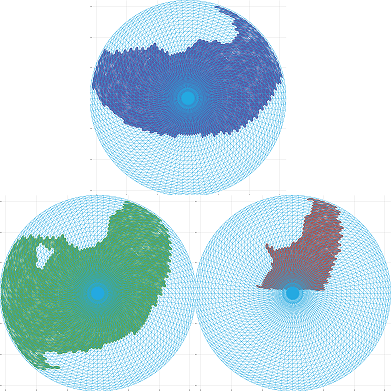
\includegraphics[width = 0.14\textwidth]{figures/real_world_exp/with_obstacle_comb}}
\subfigure[]{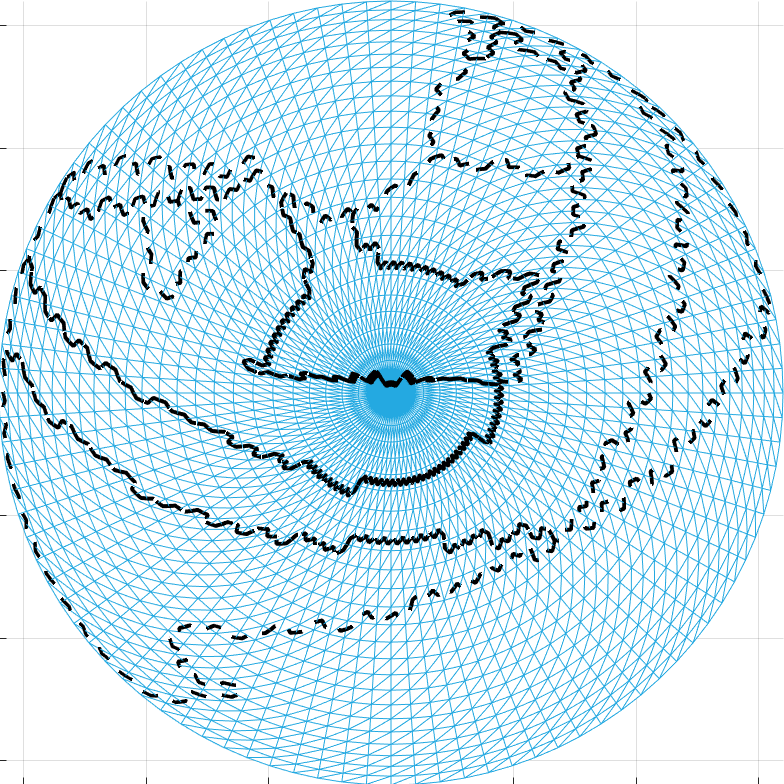
\includegraphics[width = 0.14\textwidth]{figures/real_world_exp/with_obstacle_initial_graph}}
\subfigure[]{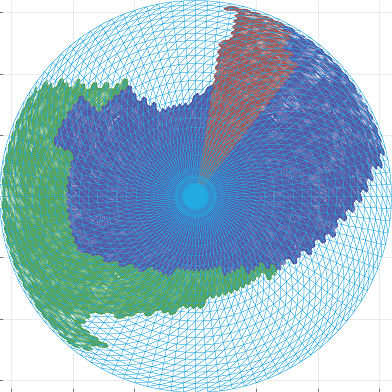
\includegraphics[width = 0.14\textwidth]{figures/real_world_exp/with_obstacle_result_graph}}
\subfigure[]{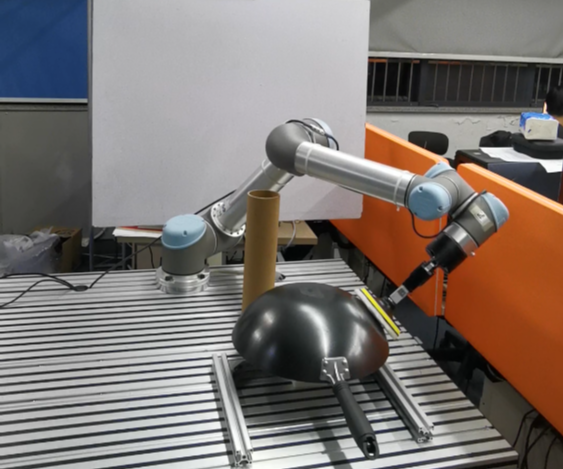
\includegraphics[width = 0.14\textwidth]{figures/real_world_exp/with_obstacle_demo_1}} \hfil
\subfigure[]{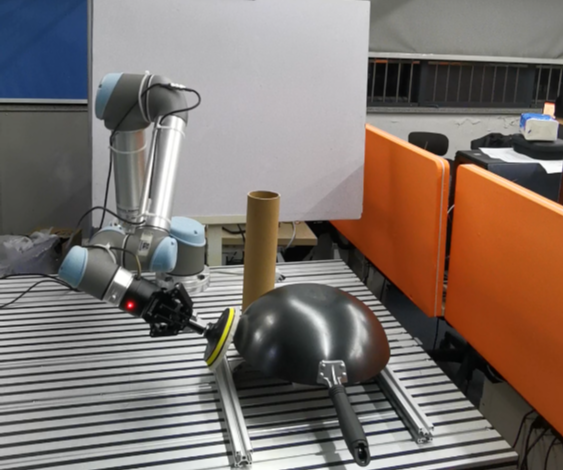
\includegraphics[width = 0.14\textwidth]{figures/real_world_exp/with_obstacle_demo_2}} \hfil
\subfigure[]{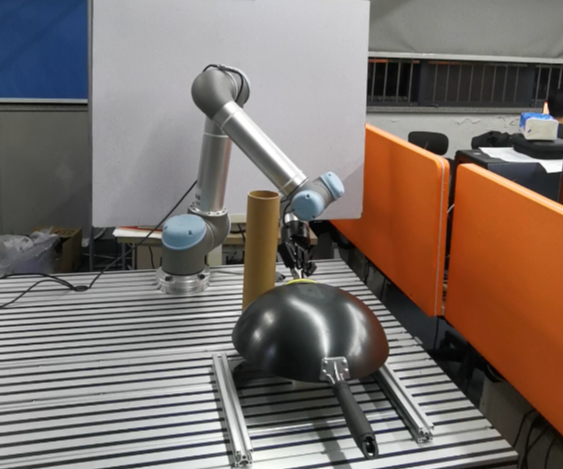
\includegraphics[width = 0.14\textwidth]{figures/real_world_exp/with_obstacle_demo_3}}
\caption{(a) Reachable coloured cells of three valid configuration, chosen by the solution in (c). 
(b) Topological graph. (c) One of the optimal solutions, requiring 2 lift-offs. 
(d),(e),(f) Example of the three kinds of configurations, where
(d) Example of the shoulder-left configuration adopted to avoid collision between the upper-arm and the obstacle. 
(e) Example of the wrist above the fore-arm configuration, so that the wrist avoids colliding with the fore-arm. 
(f) An example of the only valid configuration to cover the points in the brown cell, situating the wrist below the fore-arm.}
\label{fig:realworld_obstacle}
\end{figure}

To this end, instead of considering the design of a coverage path in the traditional sense, this research considers the global optimal cellular decomposition problem in joint-space to assemble minimum sets that guarantee homogeneous joint-space configurations. In noting that IK mapping from the reachable points in the workspace to a single set of configurations is injective, 
%since there is no non-singular path connecting two configurations whose EEs are at a same point. As such, 
colouring a point in the surface to be covered means selecting a given IK solution for it, and the planning problem is transfered to designing a colour scheme for a topological configuration graph. %In that way, the key concern is joint-space continuity of the cells. 
The proposed scheme thus provides two relevant conributions to the CPP problem in relation to optimal discontinuities:  
(a) proof that the least number of discontinuities, or ``lift-offs'', is independent of the choice of coverage path, and (b)
suggesting a novel cellular decomposition strategy to efficiently discard of equivalent cells. In proving 
that the total number of different cellular decompositions is finite, all optimal solutions are demonstrated finitely solvable. 

After applying any conventional CPP algorithm in each resulting cell, the nominated algorithm thus generates a coverage path containing the least number of discontinuities. As a direct corollary, the scheme can be applied to any other cellular decomposition methods in the literature (e.g. Morse-based), to produce the least number of discontinuities obeying the given cellular decomposition method. It can also be exploited as a criterion to evaluate placement of a manipulator or object in the workspace for minimal lift-off coverage paths. A systematic methodology to resolve this topic is left for future work.
Extensive simulation and a real-world implementation on a 5 DoF manipulator in realistic conditions are presented, supplemented by a detailed video. 
A comprehensive comparison with other geometric CPPs show the merit of the scheme and proves the validity of the proposed strategy in producing highly effective coverage paths.




% An example of a floating figure using the graphicx package.
% Note that \label must occur AFTER (or within) \caption.
% For figures, \caption should occur after the \includegraphics.
% Note that IEEEtran v1.7 and later has special internal code that
% is designed to preserve the operation of \label within \caption
% even when the captionsoff option is in effect. However, because
% of issues like this, it may be the safest practice to put all your
% \label just after \caption rather than within \caption{}.
%
% Reminder: the "draftcls" or "draftclsnofoot", not "draft", class
% option should be used if it is desired that the figures are to be
% displayed while in draft mode.
%
%\begin{figure}[!t]
%\centering
%\includegraphics[width=2.5in]{myfigure}
% where an .eps filename suffix will be assumed under latex, 
% and a .pdf suffix will be assumed for pdflatex; or what has been declared
% via \DeclareGraphicsExtensions.
%\caption{Simulation results for the network.}
%\label{fig_sim}
%\end{figure}

% Note that the IEEE typically puts floats only at the top, even when this
% results in a large percentage of a column being occupied by floats.


% An example of a double column floating figure using two subfigures.
% (The subfig.sty package must be loaded for this to work.)
% The subfigure \label commands are set within each subfloat command,
% and the \label for the overall figure must come after \caption.
% \hfil is used as a separator to get equal spacing.
% Watch out that the combined width of all the subfigures on a 
% line do not exceed the text width or a line break will occur.
%
%\begin{figure*}[!t]
%\centering
%\subfloat[Case I]{\includegraphics[width=2.5in]{box}%
%\label{fig_first_case}}
%\hfil
%\subfloat[Case II]{\includegraphics[width=2.5in]{box}%
%\label{fig_second_case}}
%\caption{Simulation results for the network.}
%\label{fig_sim}
%\end{figure*}
%
% Note that often IEEE papers with subfigures do not employ subfigure
% captions (using the optional argument to \subfloat[]), but instead will
% reference/describe all of them (a), (b), etc., within the main caption.
% Be aware that for subfig.sty to generate the (a), (b), etc., subfigure
% labels, the optional argument to \subfloat must be present. If a
% subcaption is not desired, just leave its contents blank,
% e.g., \subfloat[].


% An example of a floating table. Note that, for IEEE style tables, the
% \caption command should come BEFORE the table and, given that table
% captions serve much like titles, are usually capitalized except for words
% such as a, an, and, as, at, but, by, for, in, nor, of, on, or, the, to
% and up, which are usually not capitalized unless they are the first or
% last word of the caption. Table text will default to \footnotesize as
% the IEEE normally uses this smaller font for tables.
% The \label must come after \caption as always.
%
%\begin{table}[!t]
%% increase table row spacing, adjust to taste
%\renewcommand{\arraystretch}{1.3}
% if using array.sty, it might be a good idea to tweak the value of
% \extrarowheight as needed to properly center the text within the cells
%\caption{An Example of a Table}
%\label{table_example}
%\centering
%% Some packages, such as MDW tools, offer better commands for making tables
%% than the plain LaTeX2e tabular which is used here.
%\begin{tabular}{|c||c|}
%\hline
%One & Two\\
%\hline
%Three & Four\\
%\hline
%\end{tabular}
%\end{table}


% Note that the IEEE does not put floats in the very first column
% - or typically anywhere on the first page for that matter. Also,
% in-text middle ("here") positioning is typically not used, but it
% is allowed and encouraged for Computer Society conferences (but
% not Computer Society journals). Most IEEE journals/conferences use
% top floats exclusively. 
% Note that, LaTeX2e, unlike IEEE journals/conferences, places
% footnotes above bottom floats. This can be corrected via the
% \fnbelowfloat command of the stfloats package.




% if have a single appendix:
%\appendix[Proof of the Zonklar Equations]
% or
%\appendix  % for no appendix heading
% do not use \section anymore after \appendix, only \section*
% is possibly needed

% use appendices with more than one appendix
% then use \section to start each appendix
% you must declare a \section before using any
% \subsection or using \label (\appendices by itself
% starts a section numbered zero.)
%


%\appendices
%\section{Proof of the First Zonklar Equation}
%Appendix one text goes here.
%
%% you can choose not to have a title for an appendix
%% if you want by leaving the argument blank
%\section{}
%Appendix two text goes here.


% use section* for acknowledgment
\section*{Acknowledgment}
This work was supported in part by the National Key Research and Development Program of China under Grant 2018YFB1309300 and in part by the National Nature Science Foundation of China under Grant U1609210 and Grant 61903332. 

\bibliographystyle{ieeetr} %% setting the cite style
\bibliography{IEEEabrv,min_removal_revision_Tong_2}

% Can use something like this to put references on a page
% by themselves when using endfloat and the captionsoff option.
\ifCLASSOPTIONcaptionsoff
  \newpage
\fi



% trigger a \newpage just before the given reference
% number - used to balance the columns on the last page
% adjust value as needed - may need to be readjusted if
% the document is modified later
%\IEEEtriggeratref{8}
% The "triggered" command can be changed if desired:
%\IEEEtriggercmd{\enlargethispage{-5in}}

% references section

% can use a bibliography generated by BibTeX as a .bbl file
% BibTeX documentation can be easily obtained at:
% http://mirror.ctan.org/biblio/bibtex/contrib/doc/
% The IEEEtran BibTeX style support page is at:
% http://www.michaelshell.org/tex/ieeetran/bibtex/
%\bibliographystyle{IEEEtran}
% argument is your BibTeX string definitions and bibliography database(s)
%\bibliography{IEEEabrv,../bib/paper}
%
% <OR> manually copy in the resultant .bbl file
% set second argument of \begin to the number of references
% (used to reserve space for the reference number labels box)
%\begin{thebibliography}{1}
%
%\bibitem{IEEEhowto:kopka}
%H.~Kopka and P.~W. Daly, \emph{A Guide to \LaTeX}, 3rd~ed.\hskip 1em plus
%  0.5em minus 0.4em\relax Harlow, England: Addison-Wesley, 1999.
%
%\end{thebibliography}

% biography section
% 
% If you have an EPS/PDF photo (graphicx package needed) extra braces are
% needed around the contents of the optional argument to biography to prevent
% the LaTeX parser from getting confused when it sees the complicated
% \includegraphics command within an optional argument. (You could create
% your own custom macro containing the \includegraphics command to make things
% simpler here.)
%\begin{IEEEbiography}[{\includegraphics[width=1in,height=1.25in,clip,keepaspectratio]{mshell}}]{Michael Shell}
% or if you just want to reserve a space for a photo:

\vspace*{-5mm}

\begin{IEEEbiography}[{\includegraphics[width=1.1 in,height=1.25 in,clip,keepaspectratio]{figures/author_pics/tongyang_cropped}}]{Tong Yang} 
is currently pursuing the Ph.D. degree with the Institute of Cyber-Systems and Control, Department of Control Science and Engineering, Zhejiang University, Hangzhou, China. His current research interests include robot planning and control.
\end{IEEEbiography}

\vspace*{-5mm}

% if you will not have a photo at all:
\begin{IEEEbiography}[{\includegraphics[width=1.1 in,height=1.25 in,clip,keepaspectratio]{figures/author_pics/jaime_pic}}]
{Jaime Valls Miro} received his B.Eng. and M.Eng. in Computer Systems from the Valencia Polytechnic University (UPV, Spain). He received his Ph.D. in robotics and control systems from Middlesex University (UK). He is currently an Associate Professor at the Centre for Autonomous Systems in UTS (Australia). His areas of interest span across the field of robotics, most notably modelling sensor behaviours for perception and mapping, computational Intelligence in HRI , and robot navigation. 
\end{IEEEbiography}

% insert where needed to balance the two columns on the last page with
% biographies
%\newpage

\vspace*{-5mm}

\begin{IEEEbiography}[{\includegraphics[width=1.1 in,height=1.25 in,clip,keepaspectratio]{figures/author_pics/qianenlai}}]{Qianen Lai}
is currently pursuing the master degree with the Institute of Cyber-Systems and Control, Department of Control Science and Engineering, Zhejiang University, Hangzhou, China. His current research interests include robot grasping and robotics vision.
\end{IEEEbiography}

\vspace*{-5mm}

\begin{IEEEbiography}[{\includegraphics[width=1.1 in,height=1.25 in,clip,keepaspectratio]{figures/author_pics/yuewang}}]{Yue Wang}
 is currently a Post-Doctotral Fellow with the Institute of Cyber-Systems and Control, Department of Control Science and Engineering, Zhejiang University, Hangzhou, China. His current research interests include mobile robotics and robot perception.
\end{IEEEbiography}

\vspace*{-5mm}

\begin{IEEEbiography}[{\includegraphics[width=1.1 in,height=1.25 in,clip,keepaspectratio]{figures/author_pics/rongxiong}}]{Rong Xiong}
is currently a Professor with the Institute of Cyber-Systems and Control, Department of Control Science and Engineering, Zhejiang University, Hangzhou, China. Her current research interests include robot planning and robotics vision.
\end{IEEEbiography}

% You can push biographies down or up by placing
% a \vfill before or after them. The appropriate
% use of \vfill depends on what kind of text is
% on the last page and whether or not the columns
% are being equalized.

\vfill

% Can be used to pull up biographies so that the bottom of the last one
% is flush with the other column.
%\enlargethispage{-5in}

% that's all folks
\end{document}


